% Options for packages loaded elsewhere
\PassOptionsToPackage{unicode}{hyperref}
\PassOptionsToPackage{hyphens}{url}
%
\documentclass[
]{book}
\usepackage{amsmath,amssymb}
\usepackage{iftex}
\ifPDFTeX
  \usepackage[T1]{fontenc}
  \usepackage[utf8]{inputenc}
  \usepackage{textcomp} % provide euro and other symbols
\else % if luatex or xetex
  \usepackage{unicode-math} % this also loads fontspec
  \defaultfontfeatures{Scale=MatchLowercase}
  \defaultfontfeatures[\rmfamily]{Ligatures=TeX,Scale=1}
\fi
\usepackage{lmodern}
\ifPDFTeX\else
  % xetex/luatex font selection
\fi
% Use upquote if available, for straight quotes in verbatim environments
\IfFileExists{upquote.sty}{\usepackage{upquote}}{}
\IfFileExists{microtype.sty}{% use microtype if available
  \usepackage[]{microtype}
  \UseMicrotypeSet[protrusion]{basicmath} % disable protrusion for tt fonts
}{}
\makeatletter
\@ifundefined{KOMAClassName}{% if non-KOMA class
  \IfFileExists{parskip.sty}{%
    \usepackage{parskip}
  }{% else
    \setlength{\parindent}{0pt}
    \setlength{\parskip}{6pt plus 2pt minus 1pt}}
}{% if KOMA class
  \KOMAoptions{parskip=half}}
\makeatother
\usepackage{xcolor}
\usepackage{longtable,booktabs,array}
\usepackage{calc} % for calculating minipage widths
% Correct order of tables after \paragraph or \subparagraph
\usepackage{etoolbox}
\makeatletter
\patchcmd\longtable{\par}{\if@noskipsec\mbox{}\fi\par}{}{}
\makeatother
% Allow footnotes in longtable head/foot
\IfFileExists{footnotehyper.sty}{\usepackage{footnotehyper}}{\usepackage{footnote}}
\makesavenoteenv{longtable}
\usepackage{graphicx}
\makeatletter
\def\maxwidth{\ifdim\Gin@nat@width>\linewidth\linewidth\else\Gin@nat@width\fi}
\def\maxheight{\ifdim\Gin@nat@height>\textheight\textheight\else\Gin@nat@height\fi}
\makeatother
% Scale images if necessary, so that they will not overflow the page
% margins by default, and it is still possible to overwrite the defaults
% using explicit options in \includegraphics[width, height, ...]{}
\setkeys{Gin}{width=\maxwidth,height=\maxheight,keepaspectratio}
% Set default figure placement to htbp
\makeatletter
\def\fps@figure{htbp}
\makeatother
\setlength{\emergencystretch}{3em} % prevent overfull lines
\providecommand{\tightlist}{%
  \setlength{\itemsep}{0pt}\setlength{\parskip}{0pt}}
\setcounter{secnumdepth}{5}
\usepackage{booktabs}
\usepackage{amsthm}
\makeatletter
\def\thm@space@setup{%
  \thm@preskip=8pt plus 2pt minus 4pt
  \thm@postskip=\thm@preskip
}
\makeatother
\ifLuaTeX
  \usepackage{selnolig}  % disable illegal ligatures
\fi
\usepackage[]{natbib}
\bibliographystyle{apalike}
\usepackage{bookmark}
\IfFileExists{xurl.sty}{\usepackage{xurl}}{} % add URL line breaks if available
\urlstyle{same}
\hypersetup{
  pdftitle={Tutorial on Phonetics and Speech Analysis},
  hidelinks,
  pdfcreator={LaTeX via pandoc}}

\title{Tutorial on Phonetics and Speech Analysis}
\author{true \and true}
\date{Document compiled 06 Dec 2024 14:00}

\begin{document}
\maketitle

{
\setcounter{tocdepth}{1}
\tableofcontents
}
\chapter*{Preface}\label{preface}
\addcontentsline{toc}{chapter}{Preface}

\section*{Aims}\label{aims}
\addcontentsline{toc}{section}{Aims}

In this tutorial you will learn about \textbf{acoustics} (sounds), \textbf{phonetics} (speech), and \textbf{speech analysis}.
You will learn the core concepts in these related fields, as well as the necessary practical skills for speech analysis.
The aim of this tutorial is to provide you with the phonetic insights and skills in speech analysis that you need to succesfully conduct phonetic research in your own project (e.g.~paper or thesis).

\subsection*{Under construction}\label{under-construction}
\addcontentsline{toc}{subsection}{Under construction}

This tutorial is a work in progress, resulting from an ongoing revision of an existing tutorial, and meanwhile incorporating other modules and resources.

The existing (outdated) full tutorial is still available at \url{https://resources.lab.hum.uu.nl/resources/phonetics/index.html}
.

More details on the origins of this tutorial are provided below.

\section*{How to use this tutorial}\label{how-to-use-this-tutorial}
\addcontentsline{toc}{section}{How to use this tutorial}

You will learn the most from this tutorial if you

\begin{enumerate}
\def\labelenumi{(\arabic{enumi})}
\tightlist
\item
  read the explanatory texts in this tutorial,
\item
  work through the questions and exercises provided,
\item
  practice in applying your new knowledge hands-on, with the \texttt{Praat} computer program (detailed below), and
\item
  re-read the relevant sections from this tutorial and your textbook, with the help of keywords provided per section.
\end{enumerate}

\phantomsection\label{question-intro}
\subsection*{Questions}\label{questions}
\addcontentsline{toc}{subsection}{Questions}

Text blocks such as this one will contain questions or exercises inviting you to engage with the tutorial. You will learn most if you attempt to answer these questions (preferably in writing) \emph{before} you proceed and \emph{before} you take a look at the answer provided. (These questions only work in the HTML version of the tutorial; other versions will just show both the question and answer subsequently.)

\subsubsection*{Question 0.1}\label{question-0.1}
\addcontentsline{toc}{subsubsection}{Question 0.1}

What is sound?

Answer 0.1

Sound is a type of energy that travels through a medium (such as air, water, or solid materials) in the form of waves. These sound waves are created by the vibration of objects, which causes the surrounding particles in the medium to move in a back-and-forth motion. This movement, or vibration, transfers energy through the medium, creating waves of high and low pressure.

\section*{Recommended software}\label{recommended-software}
\addcontentsline{toc}{section}{Recommended software}

In this tutorial you will work mostly with \texttt{Praat} \citep{Boersma_Weenink_2024}\footnote{The Dutch word \emph{praat} /ˈpraːt/ means ``talk''.}. This is a popular open-source program for the analysis of speech, developed by Paul Boersma and David Weenink (both at University of Amsterdam). It can be found on its own website (\url{https://www.praat.org}), where you will find a wealth of helpful documentation. \texttt{Praat} also has extensive \texttt{Help} built in, including a full tutorial.\\
There is an online forum (\url{https://groups.io/g/Praat-Users-List}), where users share their knowledge by posting questions and providing answers.

In order to install \texttt{Praat} on your computer, go to its webpage at \url{https://www.praat.org/}, and then proceed to the download page for the operating system of your computer. Follow the installation instructions on the download page for your operating system.

\phantomsection\label{tech-layout}
\subsection*{\texorpdfstring{Instructions for using \texttt{Praat}}{Instructions for using Praat}}\label{instructions-for-using-praat}
\addcontentsline{toc}{subsection}{Instructions for using \texttt{Praat}}

Text blocks such as this one will contain instructions about how to ``do'' things in \texttt{Praat}.

Options in software menus, as well as texts in on-screen buttons, will be shown \texttt{in\ this\ way}.
The notation \texttt{Main\ \textgreater{}\ Sub} means: first choose option \texttt{Main} from the main menu, after which a submenu will appear, then choose option \texttt{Sub} from the submenu.
Commands or formulas that you have to type will be shown \texttt{in\ this\ way} too. (Commands typically need to be terminated with typing \texttt{Enter} or \texttt{Return} or \texttt{␍} or \texttt{⏎} -- which however will not be specified in the instructions.)

\section*{Structure of this tutorial}\label{structure-of-this-tutorial}
\addcontentsline{toc}{section}{Structure of this tutorial}

TBA

\section*{Recommended textbooks}\label{recommended-textbooks}
\addcontentsline{toc}{section}{Recommended textbooks}

This tutorial is intended to be used in addition to one or more textbook(s) in Phonetics, to which this tutorial will provide additional background knowledge. Some excellent textbooks in Phonetics are those by
\citet{Rietveld_VanHeuven_2009} (in Dutch),
\citet{Johnson_2011},
\citet{Ladefoged_Johnson_2015},\\
\citet{Reetz_Jongman_2020}, and
\citet{Zsiga_2024}.

\section*{Details}\label{details}
\addcontentsline{toc}{section}{Details}

\subsection*{License}\label{license}
\addcontentsline{toc}{subsection}{License}

This work is licensed under the \emph{GNU GPL 3} license (for details see
\url{https://www.gnu.org/licenses/gpl-3.0.en.html}).

\subsection*{Citation}\label{citation}
\addcontentsline{toc}{subsection}{Citation}

TBA

\subsection*{Technical details}\label{technical-details}
\addcontentsline{toc}{subsection}{Technical details}

TBA

\subsection*{History}\label{history}
\addcontentsline{toc}{subsection}{History}

This work is based on an earlier tutorial (2006-2007) titled Tutorial for self study: basics of phonetics and how to use Praat by Clizia Welker and Hugo Quené. In turn, that 2007 tutorial was partly based on older texts by Hugo Quené, Denise Bruin and Mirjam Wester (1996-2000); these older texts acknowledged valuable comments and suggestions by Paul Boersma, Olga van Herwijnen, Kim Koppen, Eva Sittig, Joyce Vliegen and Mieke van Wijck.

The 2007 version of the tutorial was subsequently revised and adapted to the current version using \texttt{R\ Markdown} \citep{rmarkdown2018} and \texttt{bookdown} \citep{R-bookdown} in \href{https://www.rstudio.com}{Rstudio} by Hugo Quené in 2024.

\begin{center}\rule{0.5\linewidth}{0.5pt}\end{center}

\part*{Part I: Sounds}\label{part-part-i-sounds}
\addcontentsline{toc}{part}{Part I: Sounds}

\chapter{Sound waves}\label{ch-soundwaves}

\emph{Chapter keywords}: sound, sound wave, oscillation, propagation, longitudinal wave, transverse wave, medium, speed of sound, force, pressure, Pascal, oscillogram, frequency, Hertz, period, periodic, aperiodic, fundamental frequency, octave, amplitude, intensity, phase, Pascal, \texttt{Praat}, object, visualization, picture, figure, harmonic, overtone, timbre, Fourier, spectrum, spectral envelope, noise, impulse.

\section{Sound}\label{sound}

Sound is a type of energy that travels through a medium (such as air, water, or solid materials) in the form of waves. These sound waves are created by the vibration of objects, which causes the surrounding particles in the medium to move in a back-and-forth (oscillatory) motion. This movement, or vibration, or oscillation, transfers energy through the medium, creating waves of high and low pressure.

\section{Sound wave}\label{sec:soundwave}

A sound wave consists of pressure fluctuations caused by the molecules of the acoustic medium crowding together (compression) and moving apart (rarefaction). A sound wave is spread in all directions from the sound source; we could compare its propagation to that of a circular wave on the surface of a water basin. The molecules themselves move over a very short distance and do not travel along with the wave: instead, after the sound wave (the pressure fluctuation) has passed along, they go back to their equilibrium position.

Sound in air is different from wind. In wind, or in air flow, the air particles move from one position to another (from subtropics to equator, from lungs to mouth, from oceans to continents). In sound, however, there is no net movement of the air particles: the particles only move over a very small distance, and return to their equilibrium after the sound wave has passed. In sound waves, the distance of travel of the air molecules is only about \(10^{-11}\) to \(10^{-5}\) m, depending on the amplitude and frequency of the vibration (more about these key properties in §\ref{sec:keypropertiessound} below).
There are two kinds of waves (also depending on the acoustic medium). In \emph{longitudinal} waves (such as sound waves) the back-and-forth displacement or movement of the medium's particles is in the same direction as the propagation of the wave. In \emph{transverse} waves (such as the waves on the surface of a pond) the back-and-forth displacement of the water particles is perpendicular to the direction of propagation of the wave.\\
A stadium wave provides a clear example of a transverse wave: a group of persons (the particles) starts the wave by standing up, rising their arms, sitting down, standing up again, and so on. The persons' action is directly followed by that of their neighbours on one side, who do the same and who are again followed by their next neighbours on their side, and so on, until the wave is travelling through the whole stadium. The persons' motion (up-down) is perpendicular to the propagation of the wave (left-right along the bench).

Sound propagates in all dimensions through an acoustic medium, like an expanding sphere, which is indeed the theoretical model used to describe the sound wave propagation pattern. As the sound wave moves away from its source, more particles are involved in the pressure fluctuations. As a consequence, sound waves lose energy while travelling through the medium, as some of the energy is spent in moving increasingly more particles. Finally, sound is perceived as such when the sound wave spread by the sound source and travelling through the acoustic medium finally impinges upon the eardrum of the observer.

\section{Acoustic media}\label{acoustic-media}

Air is only one of the media through which sound can propagate. If your head is under water (as in a bath, pool, lake or sea), the water may carry sound waves from the sound source to your eardrums, and you do hear sounds. The propagation of sound waves is faster through liquids than through gases such as air: the closer the molecules of the medium (i.e.~the higher its density), the higher the speed of sound in that medium.

You can also put your ear to the ground in order to hear sounds propagated through the soil. The propagation of sound waves in solid soil is even faster than in liquids. Trying this out on dry sand on the beach, one observer noted hearing footsteps until about 25 m distant \citep[§10]{Minnaert_1970v2}.

\section{The speed of sound}\label{sec:speedofsound}

In air, the speed of sound (the speed of propagation of a sound wave, symbol \(c\)) is about 332 m/s at 0°C, about 343 m/s at 20°C, and 353 m/s at at 37°C \citep{Shadle_2010} (all for dry air at sea level).
The speed of sound in a gas such as air is affected by only two parameters:
- the ambient temperature of the gas (as shown in the numbers above),
- the composition of the gas (its mixture and the density and compressibility of its component gases), including its relative humidity: humid air holds more particles (of water), resulting in a slight increase of the speed of sound as relative humidity increases \citep{Harris_1971}\footnote{For relative humidity \textgreater30\% \citep{Harris_1971}.}.

In sea water, sound travels at about 1435 m/s, in concrete 3400 m/s, in iron (e.g.~railroad tracks) about 5100 m/s.

\section{Pressure}\label{sec:pressure}

Pressure is the amount of force on a surface. In physics, \emph{force} is defined as an influence causing an object to accelerate. It is expressed in Newton units; a Newton is the amount of force that increases the velocity of a 1-kilogram object by one meter per second (\(m/s\)). \emph{Pressure}, in turn, is defined as force per unit of area. It is measured in Pascal units, which correspond to Newton (N) per square meter (\(1\ Pa = 1\ N/m^2\)).
Under normal conditions, atmospheric air pressure is centered at 1013.25 hPa (101325 Pa, an average value\footnote{This is the standard unit of 1 atmosphere. The pressure is due to the Earth's gravition force on the Earth's atmosphere.} on a medium latitude at sea level, at 0°C), with normal meteorological fluctuations of about ± 5000 Pa. Sound wave fluctuations in air pressure are far smaller, ranging from about ±20 µPa (micropascal, or ±0.00002 Pa) at the lower threshold of hearing to about ±20 Pascal at the upper threshold of hearing. Even louder sounds, with variations in air pressure exceeding about ±20 Pascal, are painful and cause hearing damage.

\phantomsection\label{questions-soundwaves}
\section*{Questions}\label{questions-1}
\addcontentsline{toc}{section}{Questions}

\subsection*{Question 1.1}\label{question-1.1}
\addcontentsline{toc}{subsection}{Question 1.1}

Explain why a sound wave loses energy the further it is spread from the oscillation source.

Answer 1.1

The more a sound \emph{wave} moves away from the source, the more particles of the medium (e.g.~air) are involved. The amount of initial energy (spread with the source oscillation) is spread over a larger surface, of an expanding imaginary sphere, and consequently the sound wave displaces more particles. The overall amount of energy remains the same. Therefore, the energy on a single medium particle or on a single portion of the sound wave is smaller. Thus, the sound wave fades as the distance to the sound source increases.

Remember that the sound \emph{wave} travels through the medium, but the particles in the medium remain more or less in place.

\section{Oscillogram}\label{sec:oscillogram}

As explained in §\ref{sec:soundwave} above, a sound wave consists of pressure fluctuations caused by the molecules of the acoustic medium crowding together (compression) and moving apart (rarefaction). These oscillations in air pressure can be measured and visualized. (In chapter \ref{ch-soundtobytes} we'll learn how to measure, record and store a sound wave.) Here, we jump ahead and present a graphical representation of a sound wave: the \textbf{oscillogram}.
(We need the oscillogram to explain important properties of sound waves.)

In an oscillogram, the horizontal axis represents the time dimension, and the vertical axis represents the air pressure. The air pressure fluctuations (compression and rarefaction) are displayed here as vertical deviations relative to the horizontal baseline\footnote{The baseline represents the ambient average air pressure. By convention, higher air pressure is on the top side and lower air pressure at the bottom side of an oscillogram.}.
Thus an oscillogram records the back-and-forth movements of the air particles, indirectly, by recording the fluctuations in relative air pressure, at a fixed location.

\begin{figure}

{\centering 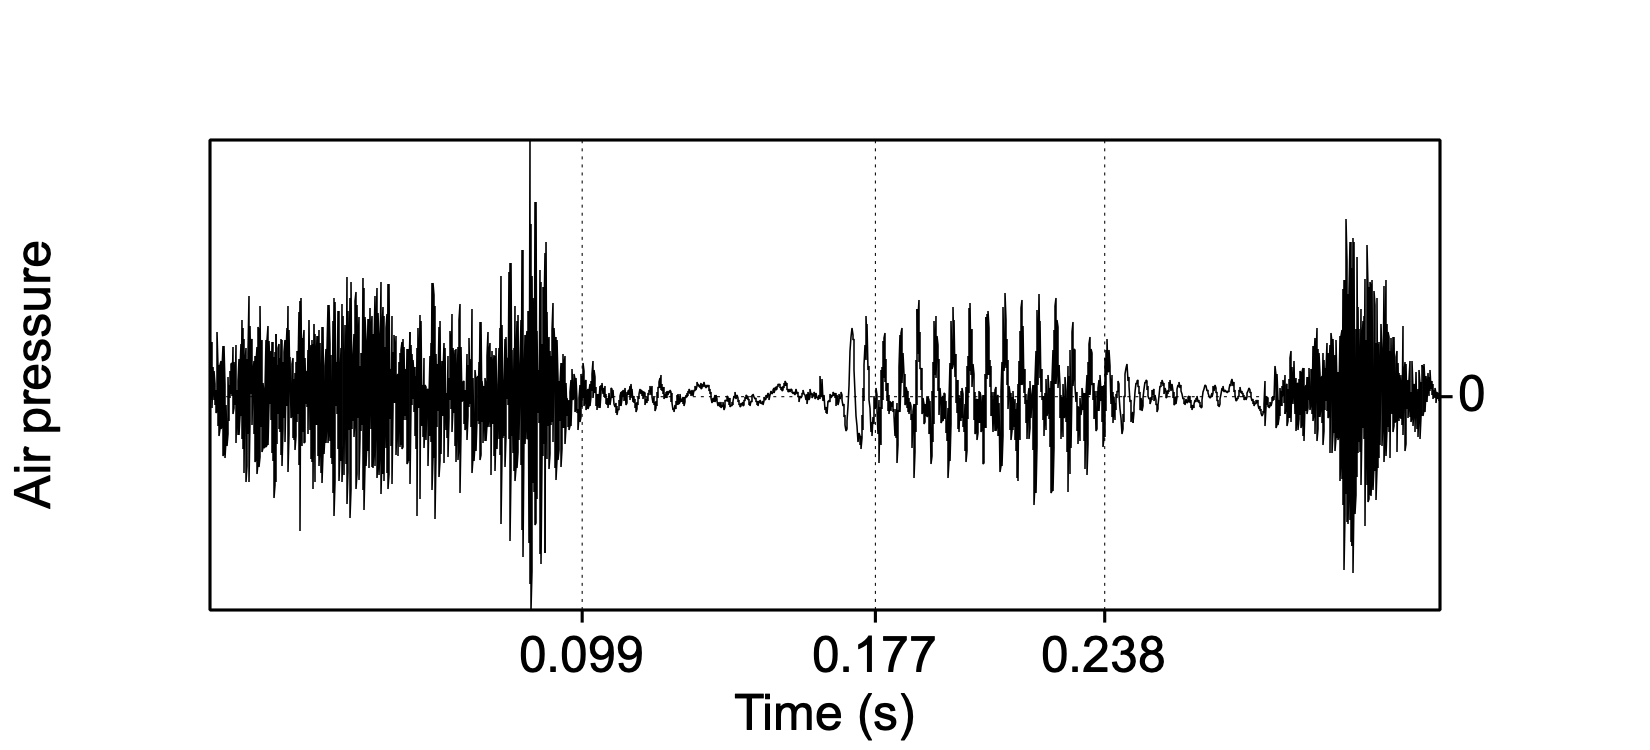
\includegraphics{figures/speech_word_oscillogram} 

}

\caption{Oscillogram of the word *speech*, with boundaries between segments.}\label{fig:speech-oscillogram}
\end{figure}

An oscillogram is comparable to a meteorologist's regular measurements of atmospheric air pressure at a fixed location --- albeit on far finer scales of time and of air pressure.

The visualisation in an oscillogram may suggest, misleadingly, that the air particles themselves dance ``up and down'' (transverse) while the sound wave travels ``from left to right'', like waves on the surface of a body of water. That is not true: sound in air travels in \emph{longitudinal} sound waves, resulting in the air pressure variations that are visualized in the oscillogram.

\section{Periodic and aperiodic sounds}\label{sec:periodicity}

There are two classes of sounds which are easily distinguishable in an oscillogram:

\begin{itemize}
\item
  \textbf{periodic} sounds, in which there is sound wave pattern that repeats itself after a particular time interval or \textbf{period} (symbol \(T\)) of a single cycle. Periodic sounds have a perceptible pitch or tone. Vowel sounds such as the /i/ in Figure \ref{fig:speech-oscillogram} (from 0.177 to 0.238 s) provide clear examples of a periodic sound.
\item
  \textbf{aperiodic} sounds, in which there is not a repetitive but instead a random pattern in the air pressure variations. Aperiodic sounds do not have a perceptible pitch but instead we hear them as noise. Some consonant sounds, e.g.~the /s/ in Figure \ref{fig:speech-oscillogram} (from 0 to 0.099 s), are clear examples of such noisy, aperiodic sounds\footnote{The clearest examples are provided by unvoiced fricative consonants, such as /f, s/.}.
\end{itemize}

\section{Key properties of a sound wave}\label{sec:keypropertiessound}

A periodic sound wave can be characterized by three key properties, which are illustrated in the oscillogram in Figure \ref{fig:example-oscillogram} and which are further discussed in the following sub-sections.

\begin{figure}

{\centering 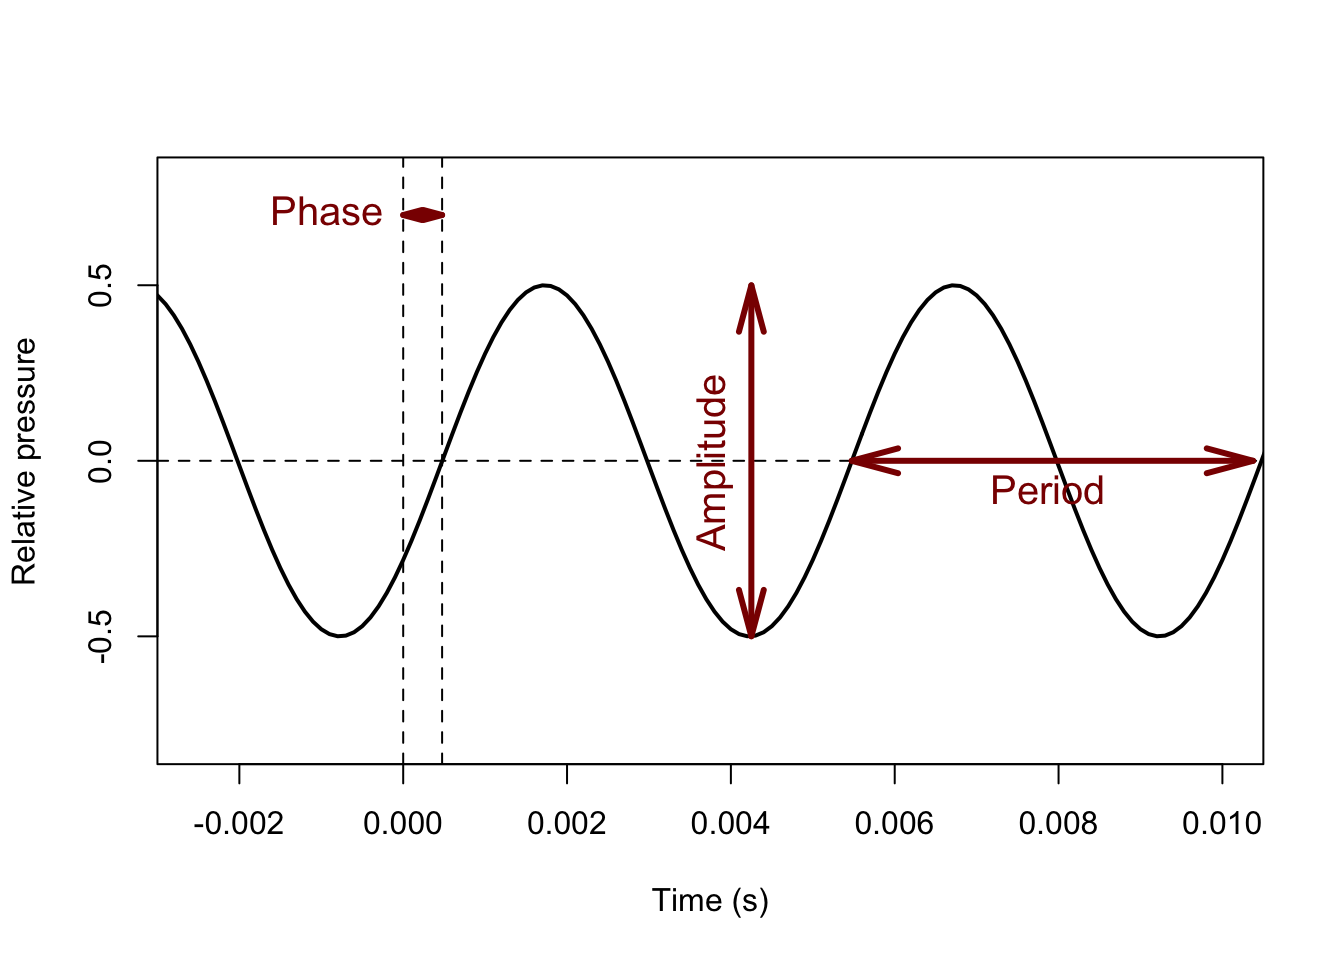
\includegraphics{TPhSA-EN_files/figure-latex/example-oscillogram-1} 

}

\caption{Oscillogram of a periodic sound (in black), with indications of the key properties frequency (1/period, see below), amplitude, and phase. The oscillogram is recorded over time (along the horizontal axis), at a fixed position in space.}\label{fig:example-oscillogram}
\end{figure}

\subsection{Frequency}\label{sec:frequency}

The frequency (symbol \(f\)) of a sound wave is the number of repeated cycles or periods (of air pressure variations) within a time interval. Only periodic sounds do have such repetitions, and thus a frequency. The frequency of a sound is perceived as its \emph{pitch} or tone. Frequency is expressed in periods per second, or Hertz units, named after Heinrich Rudolf Hertz (1857-\/--1894)\footnote{In older texts you may find `cycles per second', abbreviated `cps'.}.
Each of these periods or cycles corresponds to the repeating fluctuation between two consecutive maxima, or between corresponding `zero crossings' of adjacent periods. In Figure \ref{fig:speech-oscillogram}, in the vowel /i/, we count 14 periods in 0.065 seconds, so \(f \approx 14/0.065 \approx 215\) Hz. These periods have a duration of about \(T \approx 0.065/14 \approx 0.0046\) s\footnote{More exactly, the period \emph{is} 0.0046 s.}. Period \(T\) and frequency \(f\) are each other's inverse, so \(f=1/T\) and \(T=1/f\).

In the transverse stadium wave, the period \(T\) is the time interval between two consecutive actions of standing up by the same person (e.g.~\(T=5\) s), and frequency \(f\) is the number of actions that occur within a given time unit (e.g.~\(f=1/T=1/5\) Hz).

\subsubsection{Octave}\label{sec:octave}

An octave refers to a frequency ratio of \(1:2\) or \(2:1\), that is, doubling or halving of the frequency. An octave is the distance between 12 semitones (guitar frets or piano keys, counting black and white keys). If you sing or play a musical note (e.g.~note \texttt{A2} with \(f=110\) Hz), and then jump to the next higher octave, then the new note \texttt{A3} has a frequency of \(2 \times 110=220\) Hz. The next higher octave note \texttt{A4} has a frequency of \(2 \times 220=440\) Hz.\\
(As an aside: doubling the frequency means halving the wavelength, and vice versa, see §\ref{sec:wavelength} below).

\subsection{Amplitude}\label{sec:amplitude}

The amplitude (symbol \(A\)) of a sound wave is the extent of the variations in air pressure (due to compression and rarefaction), measured in Pascal units of pressure. With some simplification, the amplitude of a sound wave is perceived as its \emph{loudness} or `volume'. In an oscillogram, the amplitude corresponds directly to the maximum vertical displacement, that is, to the peak deviation in air pressure relative to the ambient reference pressure).

In the transverse stadium wave, the amplitude could be thought of as the extent to which persons raise their hands: the heighth of the wave crests.

In practice, the amount of energy in a (longitudinal) sound wave is better assessed in the form of \emph{intensity}, which is discussed in §\ref{sec:intensity} below.

\textbf{Study tip}: The sections on amplitude and on intensity (including decibels) are rather difficult. In first pass, just read these sections globally. After having finished the entire chapter (or more), return for a deeper second pass through these sections. Compare the explanations in these sections with those in your textbook, and then return for a third pass through these sections.

\subsubsection{RMS amplitude}\label{rms-amplitude}

How can we calculate the mean or average amplitude of a sound wave, over a particular stretch of time? We do this by squaring the amplitude values, then averaging the squared values, and then taking the Root of the Mean of the Squares. The resulting value is termed the \textbf{RMS} amplitude, and it is equivalent to the \emph{standard deviation} of the amplitude, computed over a particular stretch of time.

In a simple sinewave tone, as in Figure \ref{fig:example-oscillogram}, the RMS of the amplitude corresponds to \(0.707 \times\) the maximum or peak amplitude.

\subsection{Energy, power, intensity}\label{sec:intensity}

Amplitude is related to the pressure variations of a sound wave (with pressure defined as force per unit area; §\ref{sec:pressure}). The \emph{energy} of the sound wave is its capacity to do work, that is, to exert a force on (and thus causing displacement of) particles of the medium, that is, to propagate. Thus we want to consider the amount of acoustic energy, imparted by the vibrating sound source, and transmitted throughout the medium by causing particles to bump into each another. Energy is expressed in Joule (J) units; one Joule ``is equal to the amount of work done when a force of one newton displaces a mass through a distance of one metre in the direction of that force'' (\textless{} \url{https://en.wikipedia.org/wiki/Joule}\textgreater).

We saw earlier that we may regard the sound propagating through the medium as an imaginary expanding sphere (see §\ref{sec:soundwave}). Consider the sound of a single impulse, say a hammer hitting a nail, with air as the medium of propagation. The energy of the sound remains constant, but as the sound propagates, the imaginary sphere expands, and the original energy is distributed over a wider area of that imaginary sphere. The variations in air pressure decrease as the sphere expands, that is, as the distance to the sound source increases.

Energy is independent from the time dimension: a continuous sound having an energy of 10 J for 1 second involves as much total energy as a continuous sound having an energy of 5 J for 2 seconds. When studying sounds, however, we typically do take time into account: we are interested in the amount of energy of a sound \emph{per second}. This is termed the \emph{power} of the sound. Power is expressed in Watt (W) units; one Watt equals 1 Joule per second. By analogy, you may consider a lamp of 10 W burning for 1 hour, and another lamp of 5 W burning for 2 hours. Both lamps have consumed equal amounts of energy (in principle), but the lamp with higher power converts more energy \emph{per hour} into light: it shines brighter.

For sound waves, we are interested in the amount of power, but now expressed per unit area on the imaginary sphere of propagation of the sound wave in the medium (see §\ref{sec:soundwave}). How much acoustic energy is transferred in the wave, by particles colliding with their neigboring particles, per time and per area? This property is termed the \textbf{intensity} of the sound. Intensity is expressed in units of energy per square meter perpendicular to the direction of propagation (\(\textrm{W}/\textrm{m}^2\)).

The intensity of a sound drops off as the distance to the sound source increases\footnote{The intensity on the surface of the sphere undergoes a dropoff which can be calculated as \(I=I_s/4πr^2\), with \(I_s\) being the intensity at the source, and \(r\) being the radius of the sphere, that is, the distance from the source.}. The sound of a hammer hitting a nail has an intensity \(I/1 = I\) at a distance of \(1 \times r\), but only an intensity of \(I /2^2 = I/4\) at a double distance of \(2 \times r\).

The intensity of a sound is proportional to the maximum pressure variations of that sound, with
\[I = \frac{1}{2} \cdot \frac{p^2}{\rho \cdot c}\]
where \(p\) is the RMS amplitude of pressure variations, \(\rho\) is density of the medium (for air, \(\rho = 1.29\ \textrm{kg}/\textrm{m}^3\)) and \(c\) is speed of sound (in air, \(c = 332\ \textrm{m}/\textrm{s}\) at 0°C, see §\ref{sec:speedofsound}). A simple sine wave (as in Fig. \ref{fig:example-oscillogram}) with frequency \(f=1000\) Hz and with RMS amplitude of pressure of \(p=2 \cdot 10^{-5}\ \textrm{N}/\textrm{m}^2\) has an intensity \(I = 4.7 \cdot 10^{-13}\ \textrm{W}/\textrm{m}^2\).
Because \(1/2\) and \(\rho\) and \(c\) are approximately constant, the relationship between intensity \(I\) and air pressure \(p\) is often simplified as \(I \propto p^2\).

Experiments have shown that the sensitivity of the human ear corresponds approximately with the \emph{logarithm} of the intensity (at the eardrum). This makes it attractive to use logarithmic scales for sound pressure and for the intensity of a sound. Such a scale allows us to represent very large and very small values with equal perceptual accuracy across the scale.

\subsubsection{Logarithm}\label{sec:logarithm}

The \emph{logarithm} of a number \(x\), or \(\log(x)\), is the exponent or power to which you must raise a given base number in order to obtain \(x\). For the base number, we often use \(10\) or \(2\). So-called `natural logarithms' have \(e \approx 2.7\) as the base number, and these are often indicated as \(\ln(x)\). For example,
\[^{10}\log(1000)=3\]
since \[10^3=1000\]

One advantage of using logarithms is that multiplication of two numbers is simplified to addition of their logarithms (using a common base):
\[100 \cdot 1000 = 100000\]
\[10^2 \cdot 10^3 = 10^{2+3} = 10^5\]
\[^{10}\log(100) + ^{10}\log(1000) =2+3= ^{10}\log(100000) =5\]

Another advantage is that large \emph{ratios} (e.g.~of sound intensities or frequencies) are easier to express as logarithms:
\[10 : 1000 = 10^1 : 10^3\]
\[^{10}\log(10) : ^{10}\log(1000) = 1 : 3\]

\phantomsection\label{log1}
By definition, \(x^0=1\), and \(^x\log(1)=0\), for any base \(x\).

Intensity is perceived in an approximately logarithmic fashion: each tenfold increase of intensity (logarithm using base \(10\)) is perceived as one equal step in intensity, as further explained below. In a similar fashion, frequency too is perceived in logarithmic fashion: each twofold increase of frequency (doubling, logarithm using base \(2\)) is perceived as one equal step in frequency, viz.~by one octave (§\ref{sec:octave}).

\subsubsection{Decibel}\label{decibel}

In practice, the sound pressure or sound intensity is expressed not in absolute units, but as a \emph{ratio} relative to the sound pressure or the sound intensity of a reference sound. One of the reasons for this practice is that equal ratios are perceived as equal steps or differences\footnote{This may be clear from the piano keyboard: each doubling of frequency (ratio \(1:2\)) is perceived as one equal octave step (divided into 12 semitone keys).}

In practice, the sound pressure or intensity of a target sound is compared with some reference sound pressure or intensity, and the target-to-reference ratio is then expressed on a logarithmic scale, in \textbf{decibel} units (dB). The decibel unit is named after Alexander Graham Bell (1847-1922, inventor of the telephone).
Several different references are commonly used:

\begin{itemize}
\item
  a reference sound that has a standard RMS pressure of \(p_0 = 2 \cdot 10^{-5}\ \textrm{Pa}\), and/or a standard intensity of \(I_0 = 10^{-12}\ \textrm{W}/\textrm{m}^2\). This is the weakest sound perceived by humans\footnote{This reference is the \emph{minimal} hearing threshold, achieved only by the 1\% most sensitive listeners. The \emph{average} hearing threshold, achieved by 50\% of listeners, is at about +16 dB relative to this reference value \citep[Fig.96]{Fletcher_1953}, see below.}.
  As this reference \(p_0\) is expressed in RMS units of sound pressure (in Pascal units), ratios using this \(p_0\) as absolute reference are termed \texttt{dB\ Sound\ Pressure\ Level} or \texttt{dB(SPL)}, as in Table \ref{tab:decibels} below.\\
  (Aside: In the reference sound, the air particles move back and forth over a tiny distance, roughly the same as the size of the molecules in air! If our hearing would be just slightly more sensitive, we would just hear the constant (brown) noise of the Brownian movement of the particles in the atmosphere (see §\ref{sec:noise}).)
\item
  the smallest sound pressure perceived by a particular \emph{individual} listener (test participant, patient) at a particular frequency in a particular ear, this is called the `sensation level' (of that ear, listener, frequency). Comparisons using this relative threshold are termed \texttt{dB\ (SL)}; this allows us to present auditory stimuli with an equal subjective loudness across listeners and across ears.
\item
  the \emph{loudest} sound (highest pressure, or voltage, or intensity) that a device can process without distorting the input signal; incoming sounds are expressed in negative dB units below this reference.
\end{itemize}

For sound intensity levels:
\[L_I = 10 \cdot ^{10}\log \left( \frac{I}{I_0} \right)\]
where \(L_I\) is the level of intensity, in dB, \(I\) is the intensity of the target sound, and \(I_0\) is the intensity of the reference sound (see above), \(I_0 = 10^{-12}\ \textrm{W}/\textrm{m}^2\).\\
Working through this formula from the inside out, (1) we take the target-to-reference ratio, (2) we take the logarithm of that ratio (using 10 as base number): this is the Bel unit, and (3) we multiply by 10 to obtain \emph{deci}bel units.

For sound pressure levels, using RMS amplitude of sound pressure:
\[  L_p = 10 \cdot ^{10}\log \left( \frac{I}{I_0} \right) 
        = 10 \cdot  ^{10}\log \left( \frac{p}{p_0} \right)^2 
        = 20 \cdot  ^{10}\log \left( \frac{p}{p_0} \right) \]
where \(L_p\) is the level of sound pressure, in dB, \(p\) is the RMS amplitude of the target sound, and \(p_0\) is the RMS amplitude of the reference sound (see above), \(p_0 = 2 \cdot 10^{-5}\ \textrm{Pa}\).

A doubling of the sound pressure, that is, of the RMS amplitude (factor 2, ratio 2) means an increase of the sound pressure level by +6 dB, see footnote\footnote{\(20\cdot ^{10}\log \left( \frac{2}{1} \right) = 20 \cdot ^{10}\log (2) =  20 (0.30103) = 6.0206 \approx 6\)}.
A doubling of the intensity means an increase of the sound intensity by +3 dB, see footnote\footnote{\(10\cdot ^{10}\log \left( \frac{2}{1} \right) = 10 \cdot ^{10}\log (2) =   10 (0.30103) = 3.0103 \approx 3\)}.
By definition, a value of 0 dB means that the target sound has the same sound pressure and/or same intensity as that of the chosen reference sound.

\phantomsection\label{questions-0dB}
\subsubsection*{Question 1.2}\label{question-1.2}
\addcontentsline{toc}{subsubsection}{Question 1.2}

Check that the last sentence above holds true.

Table \ref{tab:decibels} shows some examples of sound pressure levels (in dB) under various circumstances.

\begin{longtable}[]{@{}
  >{\raggedright\arraybackslash}p{(\columnwidth - 2\tabcolsep) * \real{0.4706}}
  >{\raggedright\arraybackslash}p{(\columnwidth - 2\tabcolsep) * \real{0.5294}}@{}}
\caption{\label{tab:decibels} Examples of sound pressure levels in dB (SPL), in various situations.}\tabularnewline
\toprule\noalign{}
\begin{minipage}[b]{\linewidth}\raggedright
dB (SPL)
\end{minipage} & \begin{minipage}[b]{\linewidth}\raggedright
situation
\end{minipage} \\
\midrule\noalign{}
\endfirsthead
\toprule\noalign{}
\begin{minipage}[b]{\linewidth}\raggedright
dB (SPL)
\end{minipage} & \begin{minipage}[b]{\linewidth}\raggedright
situation
\end{minipage} \\
\midrule\noalign{}
\endhead
\bottomrule\noalign{}
\endlastfoot
0 & Reference value; absolute threshold of sine wave sound with \(f=1000\) Hz \\
16 & Average threshold of hearing for 50\% of listeners \citep[Ch.8]{Fletcher_1953} \\
20 & Leaves rustling in forest \\
27 & Outside in Hermit Basin, at the bottom of the Grand Canyon, USA \citep{Dahl_Miller_Cato_Andrew_2007} \\
30 & Whispering \\
35 & Outside in residential area, at night \\
40 & Quiet room \\
60 & Average conversation (at 1.5 m distance) \\
65 & Pedestrian city area \\
80 & Shouting, singing (at 1.5 m distance); street noise \\
92 & Outside on emergency lane of busy highway (200 cars/min, 60 mph) \citep{Dahl_Miller_Cato_Andrew_2007} \\
100 & Loud orchestra \\
120 & Threshold of pain \\
130 & Jet engine (at 30 m distance) \\
172 & Krakatoa eruption, 1893 (at 165 km distance) (\url{https://www.popsci.com/story/science/loudest-sounds-ever-measured/}) \\
192 & Loudest sound possible in air, rarefactions are vacuum (\url{https://en.wikipedia.org/wiki/Sound_pressure\#Examples_of_sound_pressure}) \\
\end{longtable}

\subsection{Phase}\label{sec:phase}

The phase of a sound wave (symbol \(\varphi\)) is the starting time of a sound wave period, relative to the duration of that period. It's easiest to explain by comparing two sounds. When listening, a single sound will arrive at our two ears at slightly different arrival times. (Unless the sound source is directly behind or in front, the sound will have a slightly longer path to travel to the further ear than to the nearer ear.) Thus the two sounds heard by the two ears will differ in phase: the starting time of a period in one ear will differ slightly from the starting time of a period in the other ear, and the difference can be expressed as the proportion of a period by which they differ.\\
The brain of the listener uses this phase difference between the two ears to estimate the direction of the sound source relative to the head. You may appreciate the effect by listening to a music record in mono or in stereo.

In addition, we use phase unconsciously to assess atmospheric and acoustic conditions. For example, when listening to a sound in a room, we hear not only the direct sound but also the indirect reflections from the floor, walls, ceiling, furniture, people, etc. The brain uses the phase relations among multiple reflections to assess the dimensions and conditions of the room.

Phase is expressed relative to the period \(T\), but it is not expressed in time (seconds) but in proportions, often expressed as degrees in the period cycle (which runs from \(0^\circ\) to \(360^\circ\)). So, a phase difference of \(\varphi=180^\circ\) and \(\varphi=0.5\) mean the same: the time difference between the two signals is half a period, whatever the duration of that period is.

In the transverse stadium wave, phase corresponds to the difference in time between the sit-down-moment of one group of persons, and the comparable sit-down-moment of another group of persons in a different section of the stadium. Imagine two waves rolling along the stadium benches: one wave on the lower benches, and a different wave on the upper benches. The two waves may be out of phase (lower and upper persons sit down at different times) or in phase (lower and upper person sit down at the same time) -- irrespective of whether the two waves have the same or different frequencies.

\phantomsection\label{questions-phase}
\subsection*{Question 1.3}\label{question-1.3}
\addcontentsline{toc}{subsection}{Question 1.3}

Continue this thought experiment, with two stadium waves having the same frequency on the lower and upper benches, and with phase \(\varphi=0.5\) between the lower and upper sections. What would the resulting wave pattern look like?

\subsection{Wavelength}\label{sec:wavelength}

The wavelength (symbol \(\lambda\)) is the length of a single cycle or period, as a distance in the medium in which the sound wave propagates, between repeated patterns in the wave. It is expressed as a distance in meters. The wavelength depends on the propagation speed \(c\) of the sound wave in m/s (see §\ref{sec:speedofsound}), and on its frequency \(f\) in Hz (see §\ref{sec:frequency}).
\[\lambda = c / f\]
\[\lambda = c \, T\]
Sounds with higher frequency have shorter wavelength, and vice versa. A periodic sound with \(f=440\) Hz has a wavelength in air of \(\lambda \approx 343/440 = 0.7795\) meter.

\begin{figure}

{\centering 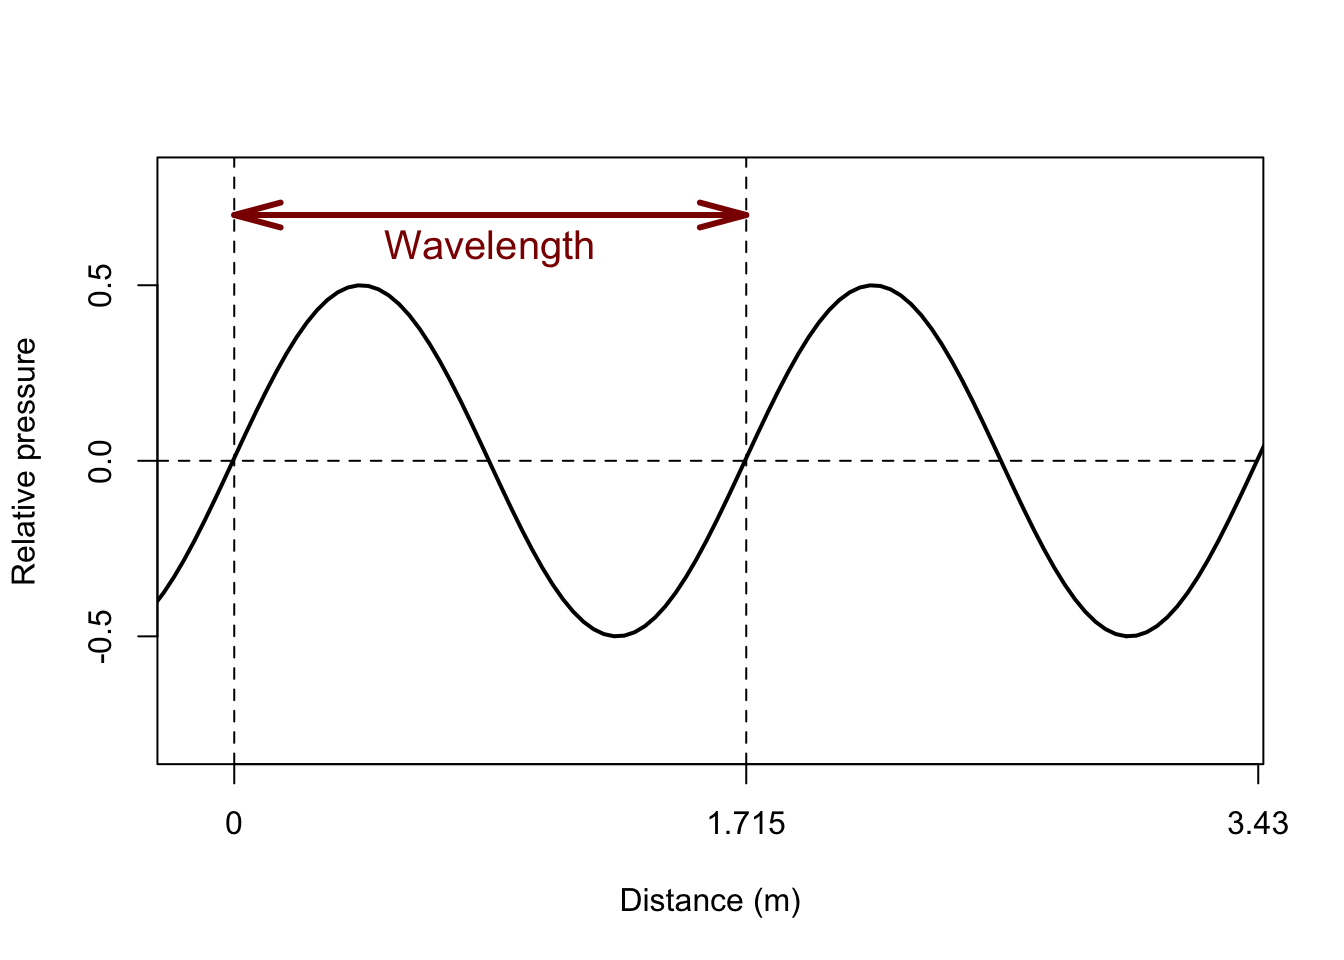
\includegraphics{TPhSA-EN_files/figure-latex/example-wavelength-1} 

}

\caption{Snapshot of the pressure of a sound wave in air, varying with distance from the sound source (along the horizontal axis). The snapshot was taken at a fixed moment in time, with c=343 m/s in the air. }\label{fig:example-wavelength}
\end{figure}

\begin{quote}
TODO adjust wavelenght plot
\end{quote}

In the transverse stadium wave, the wavelength \(\lambda\) is the distance in meters (on the same bench) between two persons in two consecutive periods who reach the highest point of their sit-stand-arms-up cycle. This is the distance the wave has traveled between the two moments at which a person repeats the same action. If we assume that \(c=10\) m/s and \(f=0.2\) Hz (as very rough estimates), we find that the wavelength \(\lambda=c/f=10/0.2=50\) meter.

\begin{center}\rule{0.5\linewidth}{0.5pt}\end{center}

\phantomsection\label{box-praatintro}
\section{\texorpdfstring{How to work with \texttt{Praat}}{How to work with Praat}}\label{sec:praatintro}

\texttt{Praat} is a computer program designed to process, analyze and visualize speech sounds.

After starting the program, \texttt{Praat} opens two windows: an \emph{Objects} window (typically on the left) and a \emph{Picture} window (typically on the right).

\subsection*{Objects}\label{objects}
\addcontentsline{toc}{subsection}{Objects}

In \texttt{Praat}, signals and derived representations are all seen as objects. Objects may have different types, e.g.~Sound, Spectrum, Pitch, etc\footnote{By convention, object types are written with a capital; this helps to distinguish physical properties (e.g.~the intensity of a sound) from the \texttt{Praat} representations of those properties (e.g.~the Intensity object computed from a Sound object, both within \texttt{Praat}).}.\\
Each type of object comes with pre-defined operations that are possible. If you select an object of a different type, then the buttons (operations) change with the object type.
As an analogy, consider the various types of objects in your room: clothing items and human bodies may be washed, food may be cooked but human bodies may not be cooked, furniture and food items may be opened but human bodies may not be opened, clothing can be inside furniture, etc. Moreover, relations between object types are also specified: for example, a plant can become a food item (by means of cooking), but a human body may not.

Before working with an object, you need to select that object, by clicking on it in the list of objects displayed in the Praat Objects window.

Objects of any type may be saved and opened using the \texttt{Save} and \texttt{Open} options in the top menu of the Objects window. This is a great way to save the objects resulting from your phonetic analyses, i.e., to save your results.

The buttons at the bottom of the Objects window are \emph{always} available for objects of any type: \texttt{Rename...}, \texttt{Copy...}, \texttt{Inspect} (to take a deeper look), \texttt{Info}, and \texttt{Remove}.

We will often work with objects of the \emph{Sound} type. Such a Sound object is a digital sound (sampled audio), which you can Play or Scale or Convert or Combine, etc. You may analyze a Sound, which will typically result in an object of a different type (e.g.~Pitch). Sound objects can be opened from disk, and saved as audio files in a wide variety of audio formats.

\subsection*{Picture window}\label{picture-window}
\addcontentsline{toc}{subsection}{Picture window}

\texttt{Praat} will draw its visualisations (figures) in its Praat Picture window. The figure will be scaled to the area with the pink boundary, the so-called viewport. By changing the viewport after drawing a part of a figure, you may obtain multiple visualizations in a single figure, as will be illustrated in this tutorial.

The combined figure in the viewport may be saved (\texttt{File\ \textgreater{}\ Save}) or printed (\texttt{File\ \textgreater{}\ Print}) in the top menu of the Praat Picture window.

You may also save the figure in a different way, as a ``recipe'' set of instructions to re-create the figure (\texttt{File\ \textgreater{}\ Save\ as\ Praat\ picture\ file}), for later reuse.

\chapter{Converting sound to bytes}\label{ch-soundtobytes}

\emph{Chapter keywords}: analog-to-digital conversion, digital-to-analog conversion, AD, DA, ADC, DAC, microphone, sound insulation, directional, filtering, sampling, sampling frequency, nyquist frequency, amplitude resolution, quantization, rounding, noise, recording level, gain, clipping, audio formats, codec, lossy, lossless, scale, fade, concatenate, chain.

\section{Overview}\label{sec:ADCoverview}

In order to process sounds by means of a computer program, or telephone, we first need to convert that sound, the variations in air pressure, to numbers that are then further processed by a computer or by a telephone device. This is a two-step process, involving at least two key components in order:

\begin{enumerate}
\def\labelenumi{(\arabic{enumi})}
\item
  the \textbf{microphone}: this device transforms variations in air pressure into matching variations in an electrical signal. The microphone has a thin membrane, and displacements of the membrane (caused by the sound pressure wave hitting the membrane) are transformed into proportional fluctuations in electric current (Ampere), electric voltage (Volt) or electric resistance (Ohm), depending on the design of the microphone. For instructions about how to handle a microphone, see the text box in §\ref{sec:microphone}) below.
  The analog electrical signal is then passed on from the microphone to\ldots{}
\item
  the \textbf{analog-to-digital-converter} (ADC): this device converts a continuous, analog electrical signal into a stream of discrete, digital numbers. The ADC measures the input signal, and reports the digital output value of that input signal. This process is also called `sampling'. Sampling a signal is done with a certain `sampling frequency' (number of measurements per second) and with a certain precision of measurement (known as `amplitude resolution'), both explained below. The result is an output stream of digital numbers (in bytes), to be handled further by computer software (e.g.~to be displayed, compressed, transmitted, stored, played back, etc.)\footnote{The input signal to be sampled often comes from a microphone, but other signals may also be sampled, e.g.~the signal coming from an electro-encephalogram (EEG) electrode.} \footnote{In a speaker's telephone, the stream of numbers (output from the ADC) constitutes the input for subsequent processing and data compression, even before speech data are transmitted to the receiving phone.}
\end{enumerate}

Very soon, whenever you want to hear sound from a computer or from a telephone connection, you will also need

\begin{enumerate}
\def\labelenumi{(\arabic{enumi})}
\setcounter{enumi}{2}
\tightlist
\item
  a \textbf{digital-to-analog-converter} (DAC): this device converts a stream of discrete, digital numbers into a continuous analog electrical signal, with a pre-specified conversion frequency and amplitude precision. The result is an output analog electrical signal, to be handled further by audio hardware (e.g.~to be amplified, sent to a loudspeaker, etc.)
\end{enumerate}

\phantomsection\label{mic-howto}
\section{How to handle a microphone}\label{sec:microphone}

\begin{itemize}
\item
  A good microphone is a very sensitive and very expensive device. Treat it with great care. Never blow into a microphone (it's far better to just say \texttt{test} or \texttt{check} or anything with plosive and fricative consonants). Do not tap on its surface.
\item
  Do not plug or unplug the microphone into/from a ``hot'' port (first set the port's input/output volume to zero, then plug/unplug).
\item
  Do not speak \emph{into} the microphone, but just over it or alongside. The microphone should measure sounds, but \emph{not} the flow of air coming out of a speaker's mouth and nose. If the microphone comes with a foam cap to dampen airflow, then use it.
\item
  Do not touch the microphone while it is working; this will result in undesired (and often loud) contact sounds in the output signal.
\end{itemize}

\section{Key parameters in AD conversion}\label{key-parameters-in-ad-conversion}

The digital signal obtained by analog-to-digital conversion is an approximation of the original (analog) sound. Two key parameters determine the accuracy of the digital approximation, and thus the quality of the digital sound recording. The first parameter is the number of samples taken per second: the \emph{sampling frequency}, and the second parameter is the number of bits used to describe the amplitude value of the sample: the \emph{amplitude resolution}. These two parameters are further explained below.

\subsection{Sampling frequency}\label{sec:samplingfrequency}

The sampling frequency (symbol \(f_s\)) is the frequency with which digital samples are taken and stored from the original analog sound. With a higher sampling frequency, the digital signal better (more closely) approximates the analog source in the time dimension, resulting in a better digital recording. The sampling frequency is expressed in samples per second, in Hertz units (cf.~§\ref{sec:frequency}). A sampling frequency of 2 kHz (2000 Hz) means that the sound is sampled \(2000 \times\) per second.

\phantomsection\label{nyquist}
The sampling frequency \(f_s\) must be at least \(2 \times\) the highest frequency \(f\) in the analog source sound. This means that the source sound may not contain any (components with) frequencies above \(f_s / 2\), the so-called `nyquist frequency'. In practice this is guaranteed by \emph{low-pass} filtering the source sound (see §\ref{sec:typesoffilters}), with the nyquist frequency as cutoff, thus removing any components with frequencies higher than the nyquist frequency, This filtering is routinely done before AD conversion, by the AD conversion hardware.

For speech, most acoustic information is contained in the frequency range up to 8 kHz. Given the previous paragraph, this means that we need a sampling frequency of at least 16 kHz\footnote{This is the typical sampling frequency in VoIP, ``wideband speech''.} or higher. In most phonetic projects, the most relevant phonetic information is contained in the frequency range up to 16 kHz, for which a sampling frequency of \(f_s = 32\) kHz\footnote{This is the standard sampling frequency for FM radio.} is adequate.
For music, relevant information may be contained in the full audible range up to 22 kHz, and the standard sampling frequency is 44.1 kHz\footnote{This is the standard sampling frequency for audio CDs.}.

\begin{itemize}
\item
  Check the sampling frequency before making a digital recording, set it to an appropriate value, write down the sampling frequency in your lab journal, and mention it in your report.
\item
  Using a higher sampling frequencies will result in proportionally larger digital sound files, which require longer processing times and more computer storage.
\end{itemize}

\subsection{Amplitude resolution}\label{amplitude-resolution}

The amplitude resolution, or quantization, refers to the number of separate steps in amplitude (voltage) that are discerned during sampling. Again, with a higher amplitude resolution, the digital signal better (more closely) approximates the analog source in the amplitude dimension, resulting in a better digital recording. The amplitude resolution is expressed in bits\footnote{1 bit or binary digit is a single digit in the binary system. A binary digit can only have 2 possible values, \(0\) or \(1\) (just as a decimal digit can have 10 possible values, \(0\) to \(9\)).} or bytes\footnote{1 byte is 8 bits, or \(2^8=256\) possible values.}.

The recorded amplitude values are discrete, and because of the ``jump'' from one discrete amplitude step to the next-higher or next-lower value, the amplitude values are ``rounded'' to some extent. This rounding or quantization results in audible noise in the digital signal. This rounding noise amounts to half a step of possible amplitude values. If we have more amplitude values (higher amplitude resolution) then the rounding off becomes less noticeable\footnote{Notice that one bit is required to record the sign of the value (positive or negative), so with 1 byte of resolution we can in principle record 256 possible amplitude values, running from -128 to +128, with rounding noise having an amplitude of \(0.5/128\) or \(1/256\) of the maximum amplitude. This corresponds to a signal-to-quantization-noise ratio of 50 dB. In practice, however, amplitude values are not stored as integer numbers but as floating numbers.}.

In phonetics, the most common amplitude resolution is 16 bits, or \(2^{16} = 65536\) different amplitude steps\footnote{This is also the standard amplitude resolution for audio CDs.}. The quantization noise has an amplitude of \(1/65636\) of the maximum amplitude; this corresponds to a signal-to-quantization-noise ratio of about 98 dB. This small amount of rounding noise is negligible.

\section{How to record a sound}\label{how-to-record-a-sound}

For any audio recording, there are a few essential precautions that you'll have to attend to, to obtain high-quality recordings suitable for subsequent analysis and re-distribution.

\phantomsection\label{recording}
\subsection{Remove non-target sounds}\label{remove-non-target-sounds}

In order to obtain a high-quality recording, it helps to attenuate all non-target sounds, in various ways:

\begin{itemize}
\tightlist
\item
  If available, use a sound-attenuating cabin or booth. The booth will help to insulate your target signal from unwanted other sounds. Close the door of the booth properly. Leave non-essential equipment (watches, phones) outside the booth.\\
  If a booth is not available, then find the quietest space available. Try using thick curtains, carpets, and cushions, and other sound-dampening materials, to improve your recording. Make lots of test recordings, listen critically, and attempt phonetic analyses before you proceed with your recordings.\\
  Background: Phonetic analyses typically aim at finding acoustic properties in the speech signal that may be related and relatable to the speaker's articulations and prosody. However, similar spectral properties (e.g.~resonances, formants, see §XXX) may also arise from acoustic reflections in the recording room, and it may be difficult or impossible to disentangle similar spectral properties coming from different origins. Hence it helps to minimize any acoustic reflections in the recording room\footnote{\emph{Frequency} and \emph{formant} measurements may be suspect if the corresponding \emph{wavelength} is a multiple of one of the dimensions of the room (see §\ref{sec:wavelength}); or if the reported frequency is below 100 Hz; or if the reliability of the frequency measurement is low.}.
\end{itemize}

\begin{quote}
TODO crossref formants.
\end{quote}

\begin{itemize}
\item
  If there is a lot of noise or non-target speech, try using a \emph{directional} microphone, which only or mostly picks up sounds coming from one direction, and which attenuates sounds from other directions. Vary the position of the microphone and make test recordings.
\item
  Switch off any non-essential equipment, and try to attenuate non-target sounds from elsewhere. Even if you cannot hear a difference, the equipment sounds and outside sounds may interfere with the target sound signal, resulting in unwanted artefacts.
\item
  Despite all these precautions, outside sounds may still interfere. This happens in particular with low-frequency signals, e.g.~due to traffic outside, elevators elsewhere in the building, and so forth. These interfering sounds are typically outside the frequency range of speech. Therefore we can easily remove them, by high-pass filtering the target speech signal, \emph{before} DA conversion.

  \begin{itemize}
  \tightlist
  \item
    Use a high-pass filter that will discard frequencies below a certain cut-off frequency (see §\ref{sec:typesoffilters}).
  \item
    Set the cut-off frequency well below the lowest possible frequency (component) in your target speech, say, a cutoff frequency of about 50 to 60 Hz.
  \end{itemize}
\end{itemize}

\subsection{Check recording level}\label{sec:recordinglevel}

\textbf{During your recording, check the level of the recording}.\\
If the recording level is too low, then the target signal is too weak, and the background noise (including quantization noise) is relatively strong. It's very difficult or impossible to fix the signal-to-noise ratio later, so you need to \textbf{fix this now}, during the recording.\\
If the recording level is too high, then the loudest portions of the target signal will be too strong, leading to ``clipping'' or distortion. It is impossible to fix this later, so you need to \textbf{fix this now}, during the recording.\\
There are several ways to adjust the level of the recording:
- by adjusting the level of the input channel (maybe called \texttt{Gain}), in your computer settings,
- by varying the distance from the sound source to the microphone (in general: the closer the better, but also depending on the type of microphone),
- in speech: by instructing the speaker to speak more loudly or more softly.

\subsection{Avoid lossy audio formats}\label{sec:avoidlossyformats}

It it tempting to record sounds digitally on smart devices which store lots of audio in compressed (lossy) formats such as MP3 or MP4. However, the lossy compression of audio data may lead to difficulties in subsequent phonetic analyses. The results may sound quite right to your ears, but details in timing or in spectral details may nevertheless have been lost in the compression. It depends on your interests and your research questions whether or not this constitutes a problem.
For phonetic research, it is generally better to record in `lossless' audio formats that do not compress the audio data, rather than in `lossy' formats. Check whether and how your smart device can make lossless recordings: if possible at all, this will probably require a deep dive into the settings on the recording device.

\subsection{\texorpdfstring{On your computer, using \texttt{Praat}}{On your computer, using Praat}}\label{on-your-computer-using-praat}

We assume that you use a computer equipped with a \textbf{microphone}, or with an analog \textbf{input port} for an analog signal coming from an external microphone. If using an external microphone, plug it into your computer (see §\ref{sec:microphone}). Check that audio input is arriving in your computer, using your computer system settings for sound input (if using an external microphone, select the appropriate channel).

There is a helpful option in \texttt{Praat}, from the \emph{main} menu (not from the Objects window menu): \texttt{Praat\ \textgreater{}\ Settings\ \textgreater{}\ Sound\ recording\ settings...} where you may adjust certain settings as needed.

\phantomsection\label{box-praatrecord}
\subsubsection{Record}\label{sec:praatrecord}

\begin{itemize}
\item
  In the Praat Objects window, select \texttt{New\ \textgreater{}\ Record\ mono\ sound}.
  In most situations it is not necessary to record stereo sounds.
\item
  Choose the appropriate sampling frequency, e.g.~22050 Hz (see §\ref{sec:samplingfrequency}). You may receive an error message if the chosen sampling frequency is incompatible with your computer.
\item
  Click \texttt{Record}, and speak a test sentence into the microphone, e.g.~\emph{The source of the huge river is the clear spring}\footnote{One of the so-called Harvard test sentences, from list 3, \url{https://en.wikipedia.org/wiki/Harvard_sentences}. In Dutch, a popular test sentence is \emph{Het leven is mooi als de zon schijnt}.}, or make a test recording of your sound source. After testing, click \texttt{Stop}.
\item
  \textbf{While recording, check the level of the recording} (§\ref{sec:recordinglevel}).\\
  In \texttt{Praat}, make sure that your recording level is in the yellow zone, with occasional peaks in the red zone, but without clipping.
\item
  Click \texttt{Play} to listen to your recording. \textbf{Repeat the recording} until the recording level is good.
\item
  Enter a name for the recording, e.g.~\texttt{river}, in the lower right corner (this name will be used within \texttt{Praat}).
\item
  Save the recording: \texttt{Save\ to\ list} (i.e., to the list of objects in the \texttt{Praat} Objects window).
\end{itemize}

Your speech recording is now an object within \texttt{Praat}.

\subsubsection{Save}\label{sec:praatsave}

For storage, you should save this object as an audio file on your computer's hard disk.

\begin{itemize}
\item
  To do so, in the \texttt{Praat} object window, select the Sound object that you just recorded. (Normally this new object has been added at the BOTTOM of the list of objects).
\item
  From the top menu, choose \texttt{Save\ \textgreater{}\ Write\ to\ WAV\ file...} or choose any of the other audio formats. Save the Sound object in a folder and under an unambiguous name that you will remember and understand a year from now -- not just \texttt{river.wav}. Note in your journal the folder and filename of your sound recording. Keep projects in separate folders on your computer.
\end{itemize}

\subsubsection{Open}\label{sec:praatopen}

\begin{itemize}
\tightlist
\item
  In order to open an audio file from your computer hard disk, from the top menu in the Objects window, choose \texttt{Open\ \textgreater{}\ Read\ from\ file...}, and pick the target audio file.
\end{itemize}

\section{How to play back a digital sound}\label{how-to-play-back-a-digital-sound}

Once again, we assume that you use a computer equipped with an analog \textbf{output port} for playing back sounds. Check that audio output is audible, using your computer system settings for sound output to your loudspeakers or headphones.

There is a helpful option in \texttt{Praat}, from the \emph{main} menu (not from the Objects window menu): \texttt{Praat\ \textgreater{}\ Settings\ \textgreater{}\ Sound\ playing\ settings...} where you may adjust certain settings as needed.

\phantomsection\label{box-praatplay}
In the Objects window, select the Sound object(s) that you want to play back. Then press the \texttt{Play} button in the Objects window. You might interrupt the playback with the \texttt{Esc} key, but this depends on your playback settings (see the paragraphs above). (If you have selected multiple Sound objects, then they will be played consecutively, \emph{without} a pause in between; see §\ref{sec:concatenate}.)

\section{How to manipulate a digital sound}\label{how-to-manipulate-a-digital-sound}

\subsection{Scale}\label{scale}

Even if you have heeded all the warnings in this chapter, it may be necessary to adjust the amplitude or intensity of your digital recording. Sample values in the digital sound will be multiplied with a certain scale factor. \texttt{Praat} has different recipes to choose this scale factor.

\phantomsection\label{box-praatscale}
\subsubsection{Scale amplitude}\label{scale-amplitude}

\texttt{Modify\ \textgreater{}\ Scale\ peak...}.\\
The amplitude scale factor is chosen so that the maximum sample value is a particular proportion \(\times\) the maximum \emph{possible} amplitude value (which in \texttt{Praat} is \(1\) by definition). Sensible values for this proportion are \(0.99\) (the default) or \(0.995\), resulting in peak values which will be \(0.2\) dB or \(0.1\) dB below the maximum possible amplitude value, respectively. (If you choose a proportion \(>1\), the result will contain clipped samples, with amplitude values exceeding the maximum possible value. This will lead to distorted sound when played back. Do not choose a proportion \(>1\) here.)

\subsubsection{Scale intensity}\label{scale-intensity}

\texttt{Modify\ \textgreater{}\ Scale\ intensity...}.\\
The amplitude scale factor is chosen so that the average \emph{intensity} of the resulting sound is the specified target intensity in dB SPL (see §\ref{sec:intensity}). \texttt{Praat} warns you that the result may contain clipped samples, with amplitude values exceeding the maximum possible value. Such clipped samples will lead to distorted sound when played back.

\phantomsection\label{fades}
\subsubsection{Fades}\label{sec:fades}

An abrupt change in amplitude may occur at the beginning and/or at the end of a sound file. Such an abrupt change will be heard as an impulse sound (see §\ref{sec:impulses}), that is, as a clicking sound. Due to the workings of the ear, this impulse may briefly mask subsequent sounds, i.e., affect the perception of subsequent sounds. In order to avoid these artefacts, it is common practice to enforce a gradual fade-in (at the onset, from zero) and fade-out (to zero). This is especially important if you intend to play back the sound to listeners.

\phantomsection\label{box-praatfades}
These smooth fades can be made in \texttt{Praat} by choosing \texttt{Modify\ \textgreater{}\ Fade\ in...} and \texttt{Modify\ \textgreater{}\ Fade\ out...}, with a fade duration of about 0.005 to 0.010 second. Samples affected by the fade are multiplied with a factor increasing from 0 to 1 during fade-in, or decreasing from 1 to 0 during fade-out.

\subsection{Concatenate}\label{sec:concatenate}

In phonetic research, we often want to construct a ``chain'' of sounds in a particular order e.g.~(1) a warning beep, (2) a silent portion of fixed duration, and (3) a speech stimulus. This can be achieved in several ways; the most basic operation is to ``concatenate'', that is, to create a ``chain'' of sound objects.

\phantomsection\label{box-praatconcatenate}
In the Praat Objects window, select the Sound objects \emph{in the order in which they are to be concatenated}, e.g.~(1) beep, (2) silence, (3) stimulus. In order to select multiple Sound objects from the list, in a specified order, press \texttt{Command} while selecting objects.~
Then choose \texttt{Combine\ \textgreater{}\ Concatenate} in the Objects window. The resulting ``chain'' of Sounds will be added to the BOTTOM of the list of objects. Remember to save this new Sound object (see §\ref{sec:praatsave}).

\chapter{Complex sounds and spectra}\label{complex-sounds-and-spectra}

\emph{Chapter keywords}: sinewave sound, complex sound, spectrum, fourier transform, fourier analysis, fast fourier transform, FFT, harmonics, fundamental, fundamental frequency, f0, overtone, component, timbre, octave, noise, white noise, brown noise, impulse.

\section{Introduction}\label{introduction}

The \emph{sine wave}, depicted in Fig. \ref{fig:example-oscillogram}, is the simplest sound possible. It is composed of the simplest back-and-forth variation or oscillation in air pressure, similar to the regular swing pattern or oscillation of a pendulum\footnote{Drawing the position of a swinging pendulum over time will result in the same figure.}. We only encounter sine wave sounds if they are artificially generated, and hardly ever in nature -- although the sound of a tuning fork comes quite close to a sinewave pattern.

By contrast, \emph{complex sounds} have more complex wave patterns. All natural periodic sounds are complex sounds. \textbf{A complex sound can be regarded as the sum of multiple sine wave sounds.} This relation has been described by the French mathematician, baron J.B.J. Fourier (1768--1830). The sine waves are termed `frequency components' of the complex sound. Each of these components has its own frequency, amplitude, and phase. In a so-called `Fourier analysis' or `Fourier Transform' of a complex sound, these frequency components are being estimated from the waveform.

If the complex sound has a repeating waveform, then we have a periodic complex sound, of which Figure \ref{fig:fourier-oscillogram} provides an example. The resulting sound has been obtained by adding three frequency components, drawn in dotted lines, of 100 Hz (\(T=.01\)) and 200 Hz (\(T=.005\)) and 400 Hz (\(T=.0025\)), respectively. Note that the frequency with which the complex sound repeats itself, 100 Hz, is the same as that of the lowest component. This lowest component is called the \emph{fundamental}, and its frequency is called the \emph{fundamental frequency} (symbol \(f_0\)) of the complex periodic sound; we hear this \(f_0\) as its pitch. The higher components are called \emph{overtones}. The fundamental and overtones are collectively called \emph{harmonics}: the fundamental is the first harmonic, the first overtone is the second harmonic, etc.
\textbf{In a periodic complex sound, the frequencies of the overtones are integer multiples of the fundamental.}

\begin{quote}
TODO crossref pitch, missing fundamental
\end{quote}

Typical examples of periodic complex sounds are the vowel sounds in normal speech. The properties of a periodic complex sound depend on the amplitudes, frequencies and phases of its component harmonics.

\begin{figure}

{\centering 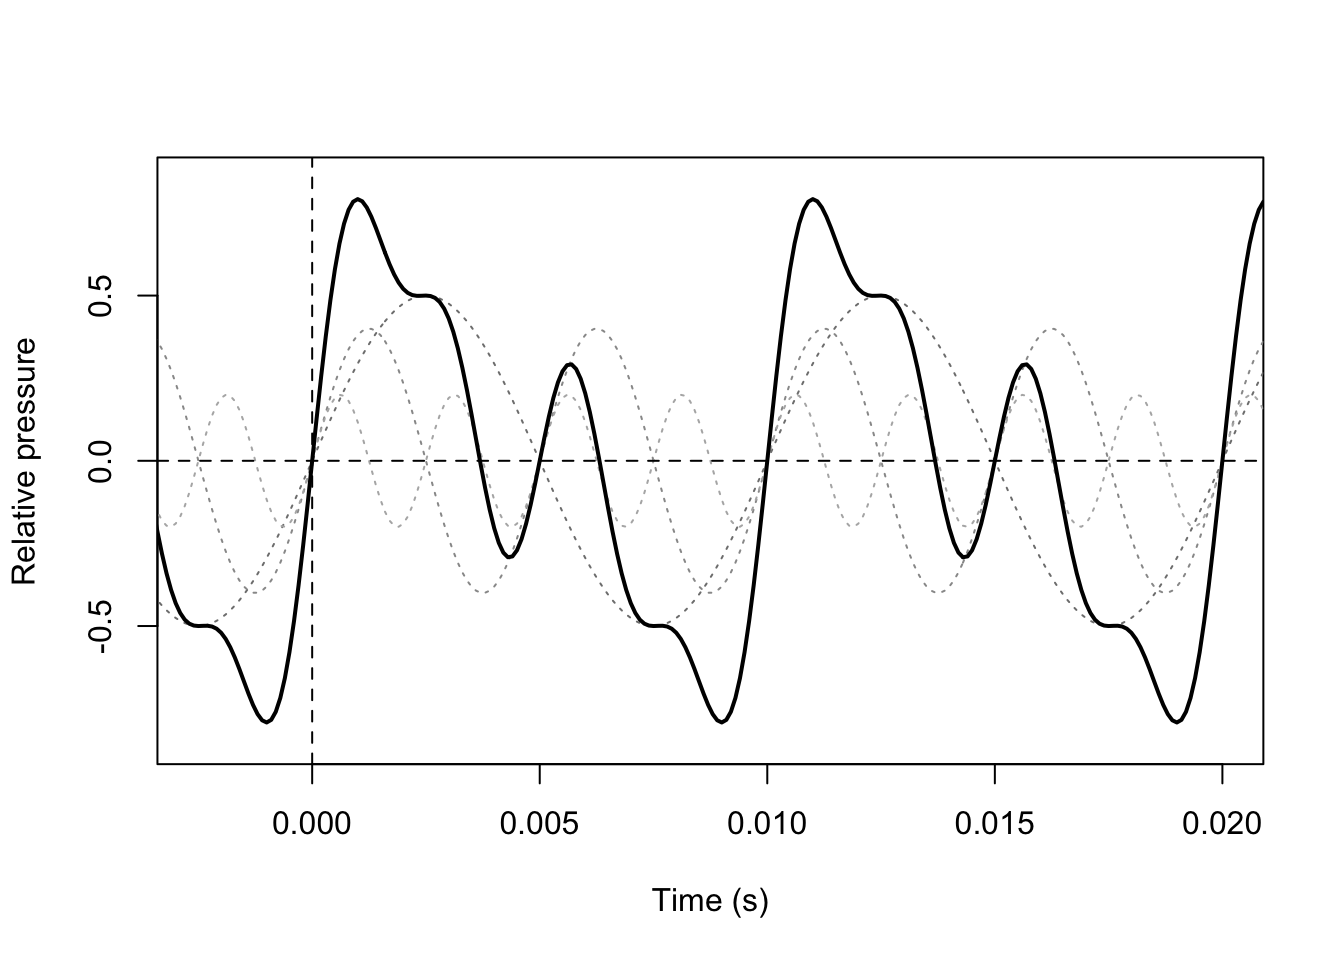
\includegraphics{TPhSA-EN_files/figure-latex/fourier-oscillogram-1} 

}

\caption{Oscillograms of three sinewave sounds and their resulting complex periodic sound.}\label{fig:fourier-oscillogram}
\end{figure}

\subsection{Timbre}\label{timbre}

Two periodic complex sounds, having the same overall amplitude and fundamental frequency, may differ strongly in their character.
The general name for this property is \emph{timbre}.
Timbre depends on the relative amplitudes of the harmonics, and hence very many different timbres are possible.
For aperiodic sounds, timbre also depends on the relative amplitudes of the (infinitely many) frequency components.
A sound may have a dull or sharp timbre, or rich or thin, warm or metallic. The difference between distinct vowels, such as /a/ vs.~/i/, spoken by the same person at the same pitch and amplitude, is also a matter of timbre, as is the difference between similar but distinct consonant sounds, such as /s/ vs.~/ʃ/.

Timbre is not a one-dimensional property of a sound (as frequency and amplitude are), but a multi-dimensional property.

\section{Spectrum}\label{spectrum}

A sound can be represented in two equivalent ways: as a function of time (in an oscillogram), or as a function of frequency. The latter representation is called a \emph{spectrum}.

Figure \ref{fig:complex100n200n400} shows an oscillogram on the left (of the same complex sound as shown in Fig. \ref{fig:fourier-oscillogram}, and its matching spectrum on the right. The spectrum shows the amplitude (along the vertical axis) of each frequency component (along horizontal axis)\footnote{Here, the phase of the frequency components is ignored.}. Hence, a spectrum shows the frequency and amplitude of each component.

\begin{figure}

{\centering 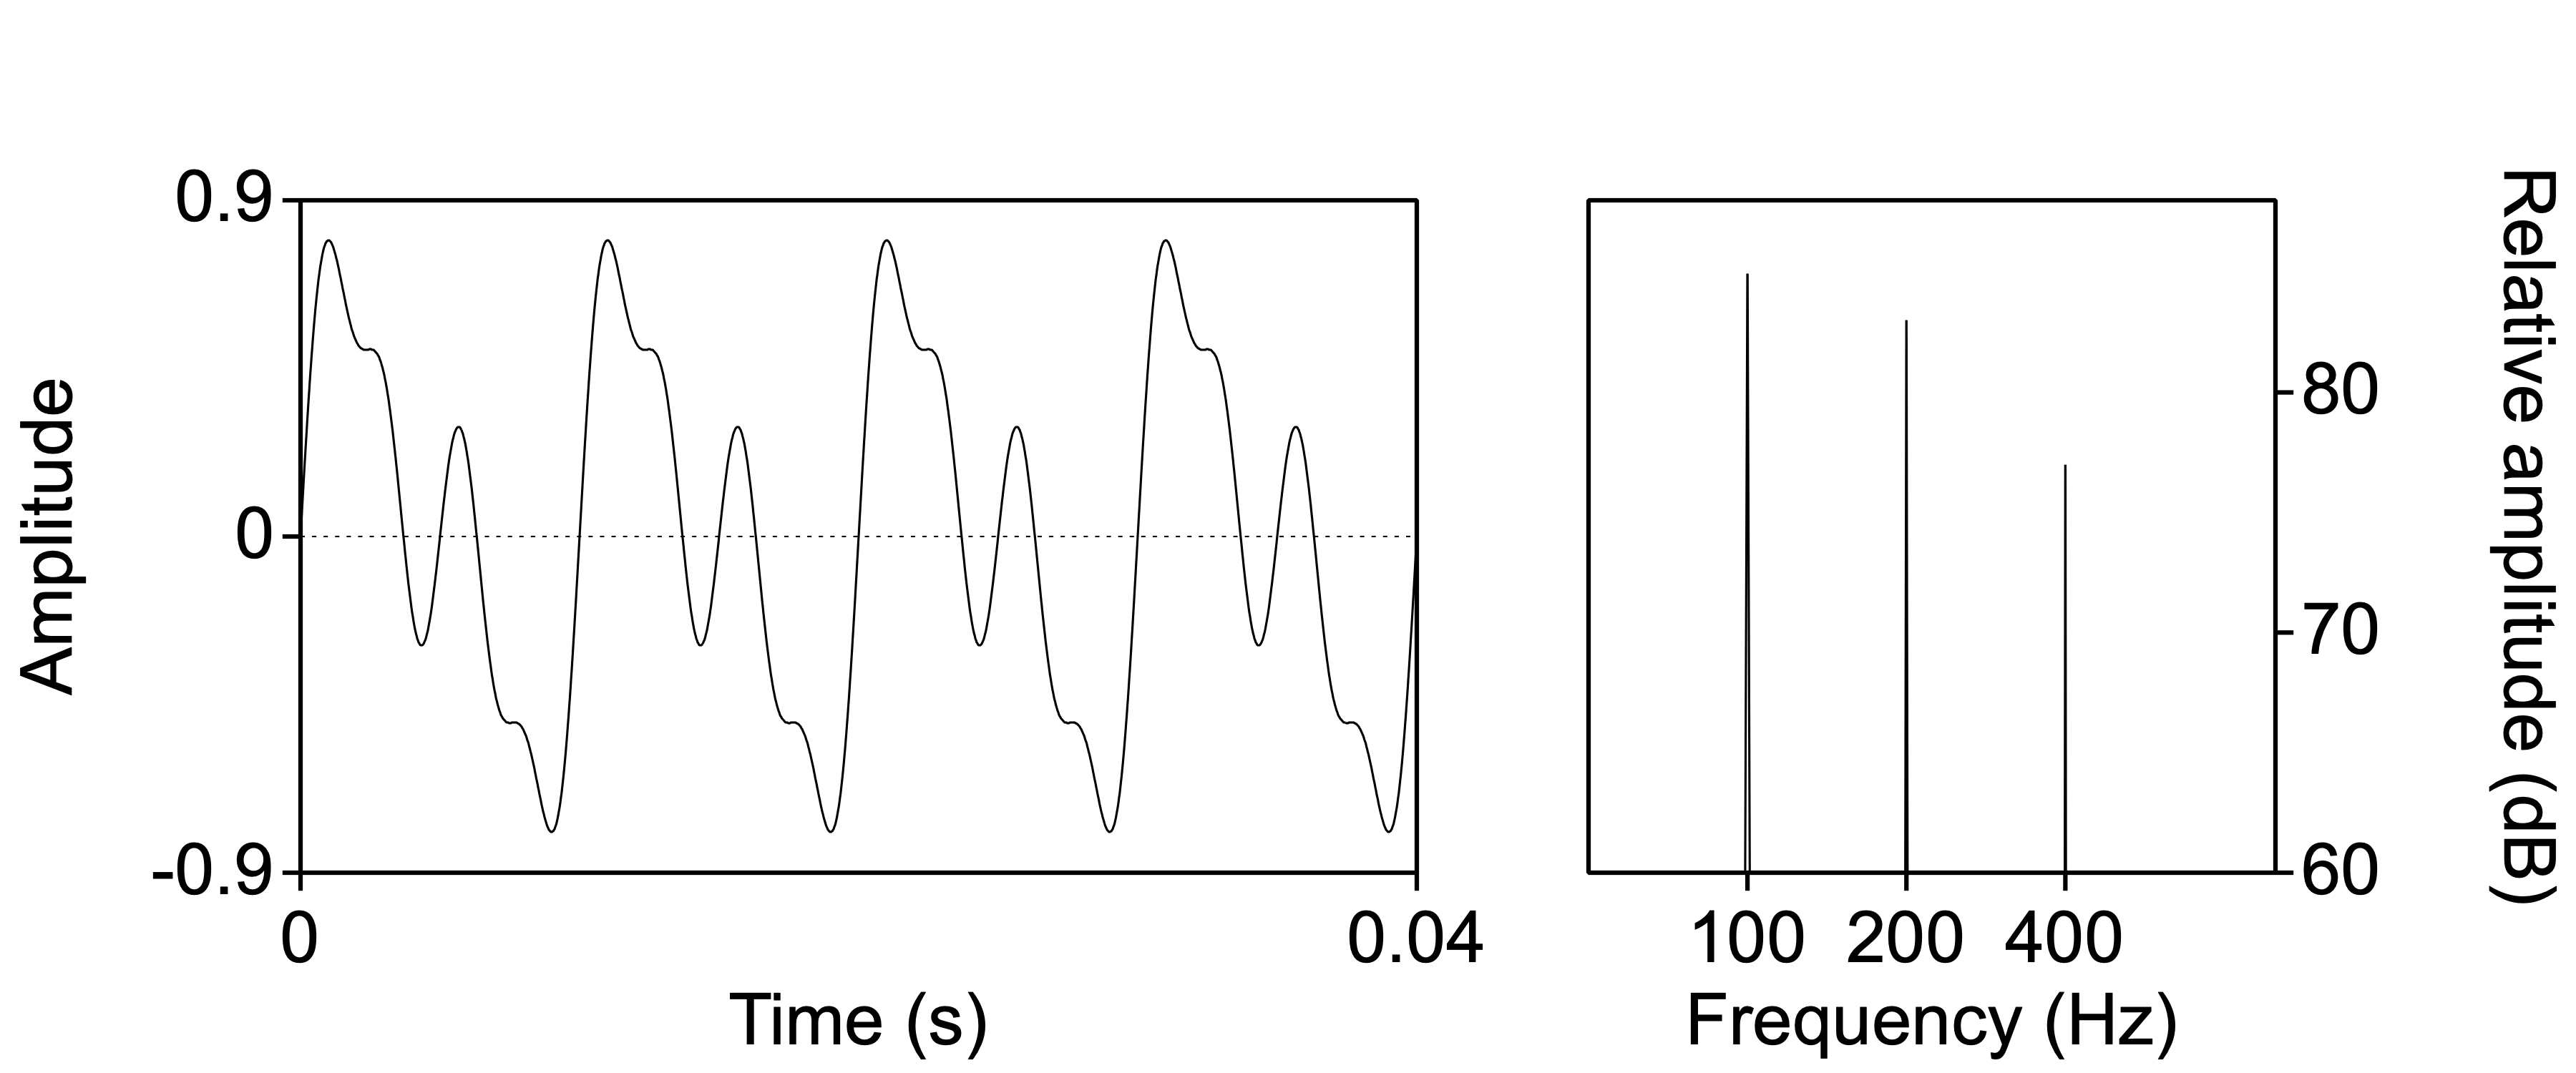
\includegraphics{figures/complex100n200n400} 

}

\caption{Oscillogram (left) and spectrum (right) of a complex periodic sound.}\label{fig:complex100n200n400}
\end{figure}

\phantomsection\label{questions-spectrum}
\subsection*{Questions}\label{questions-2}
\addcontentsline{toc}{subsection}{Questions}

\subsubsection*{Question 3.1}\label{question-3.1}
\addcontentsline{toc}{subsubsection}{Question 3.1}

Draw the spectrum of a sinewave sound with a frequency of 450 Hz and an amplitude of 40 dB SPL.

\phantomsection\label{box-praatspectrum}
\subsection{\texorpdfstring{How to obtain a spectrum in \texttt{Praat}}{How to obtain a spectrum in Praat}}\label{how-to-obtain-a-spectrum-in-praat}

\begin{itemize}
\item
  In the \texttt{Praat} object window, select a Sound object.
\item
  Next, in the \texttt{Praat} object window, choose \texttt{Analyse\ spectrum\ \textgreater{}} and then \texttt{To\ Spectrum...}.
\item
  \texttt{Praat} offers two versions, regular and fast, of the Fourier analysis to estimate a spectrum. The faster version of the Fourier transform is termed `Fast Fourier Transform' or FFT, and it requires significantly fewer computations. FFT requires that the number of samples to be analysed is a power of \(2\). If you choose the \texttt{Fast} version by ticking the box, then \texttt{Praat} adds zeroes to your sound in order to meet this requirement.
\item
  The result is a Spectrum object calculated over the entire Sound (plus additional zeroes, in FFT), and this Spectrum object is added at the bottom of the list of objects.
\item
  Remember to \texttt{Save} this Spectrum object if you wish.
\item
  As the spectral representation (spectrum, horizontal axis is frequency) is equivalent with the temporal representation (oscillogram, horizontal axis is time), the Spectrum object may be reconverted again into Sound, by means of ``inverse fourier transform''.
  To do so, select the Spectrum object, select button \texttt{Sound\ \textgreater{}} and then \texttt{To\ Sound}.
\end{itemize}

\section{Spectra of aperiodic sounds}\label{spectra-of-aperiodic-sounds}

Stable noise and brief impulses are two types of aperiodic signals (§\ref{sec:periodicity}): the variations in air pressure do not follow a regular periodic pattern\footnote{Or, you might say that the period is infinitely long.}. Aperiodic sounds do not have a fundamental frequency (because there is no regular period), and their phase is undefined, but aperiodic sounds do have an amplitude and a spectral composition.

\subsection{Noise}\label{sec:noise}

First we discuss \emph{stable} aperiodic sounds: \textbf{noise}. You might say that a noisy sound has an infinite number of frequency components. That is, the components are not only harmonics of the fundamental frequency (as with periodic complex sounds), but may be found at \emph{every} frequency. The relative amplitudes of the many frequency components determines the timbre of the noise.

In \emph{white noise}, all frequency components are equally strong\footnote{This is called `white' noise by analogy with white light, in which all frequency components in the visible part of the electromagnetic spectrum are equally strong.}, and thus the spectral envelope is flat.
In so-called \emph{brown noise}, the spectral envelope decreases by \(-6\) dB per octave, so that lower frequencies are more dominant than higher frequencies. Because this spectral envelope resembles that of speech, brown noise is often used in phonetic research whenever we need to mask speech.

\begin{figure}

{\centering 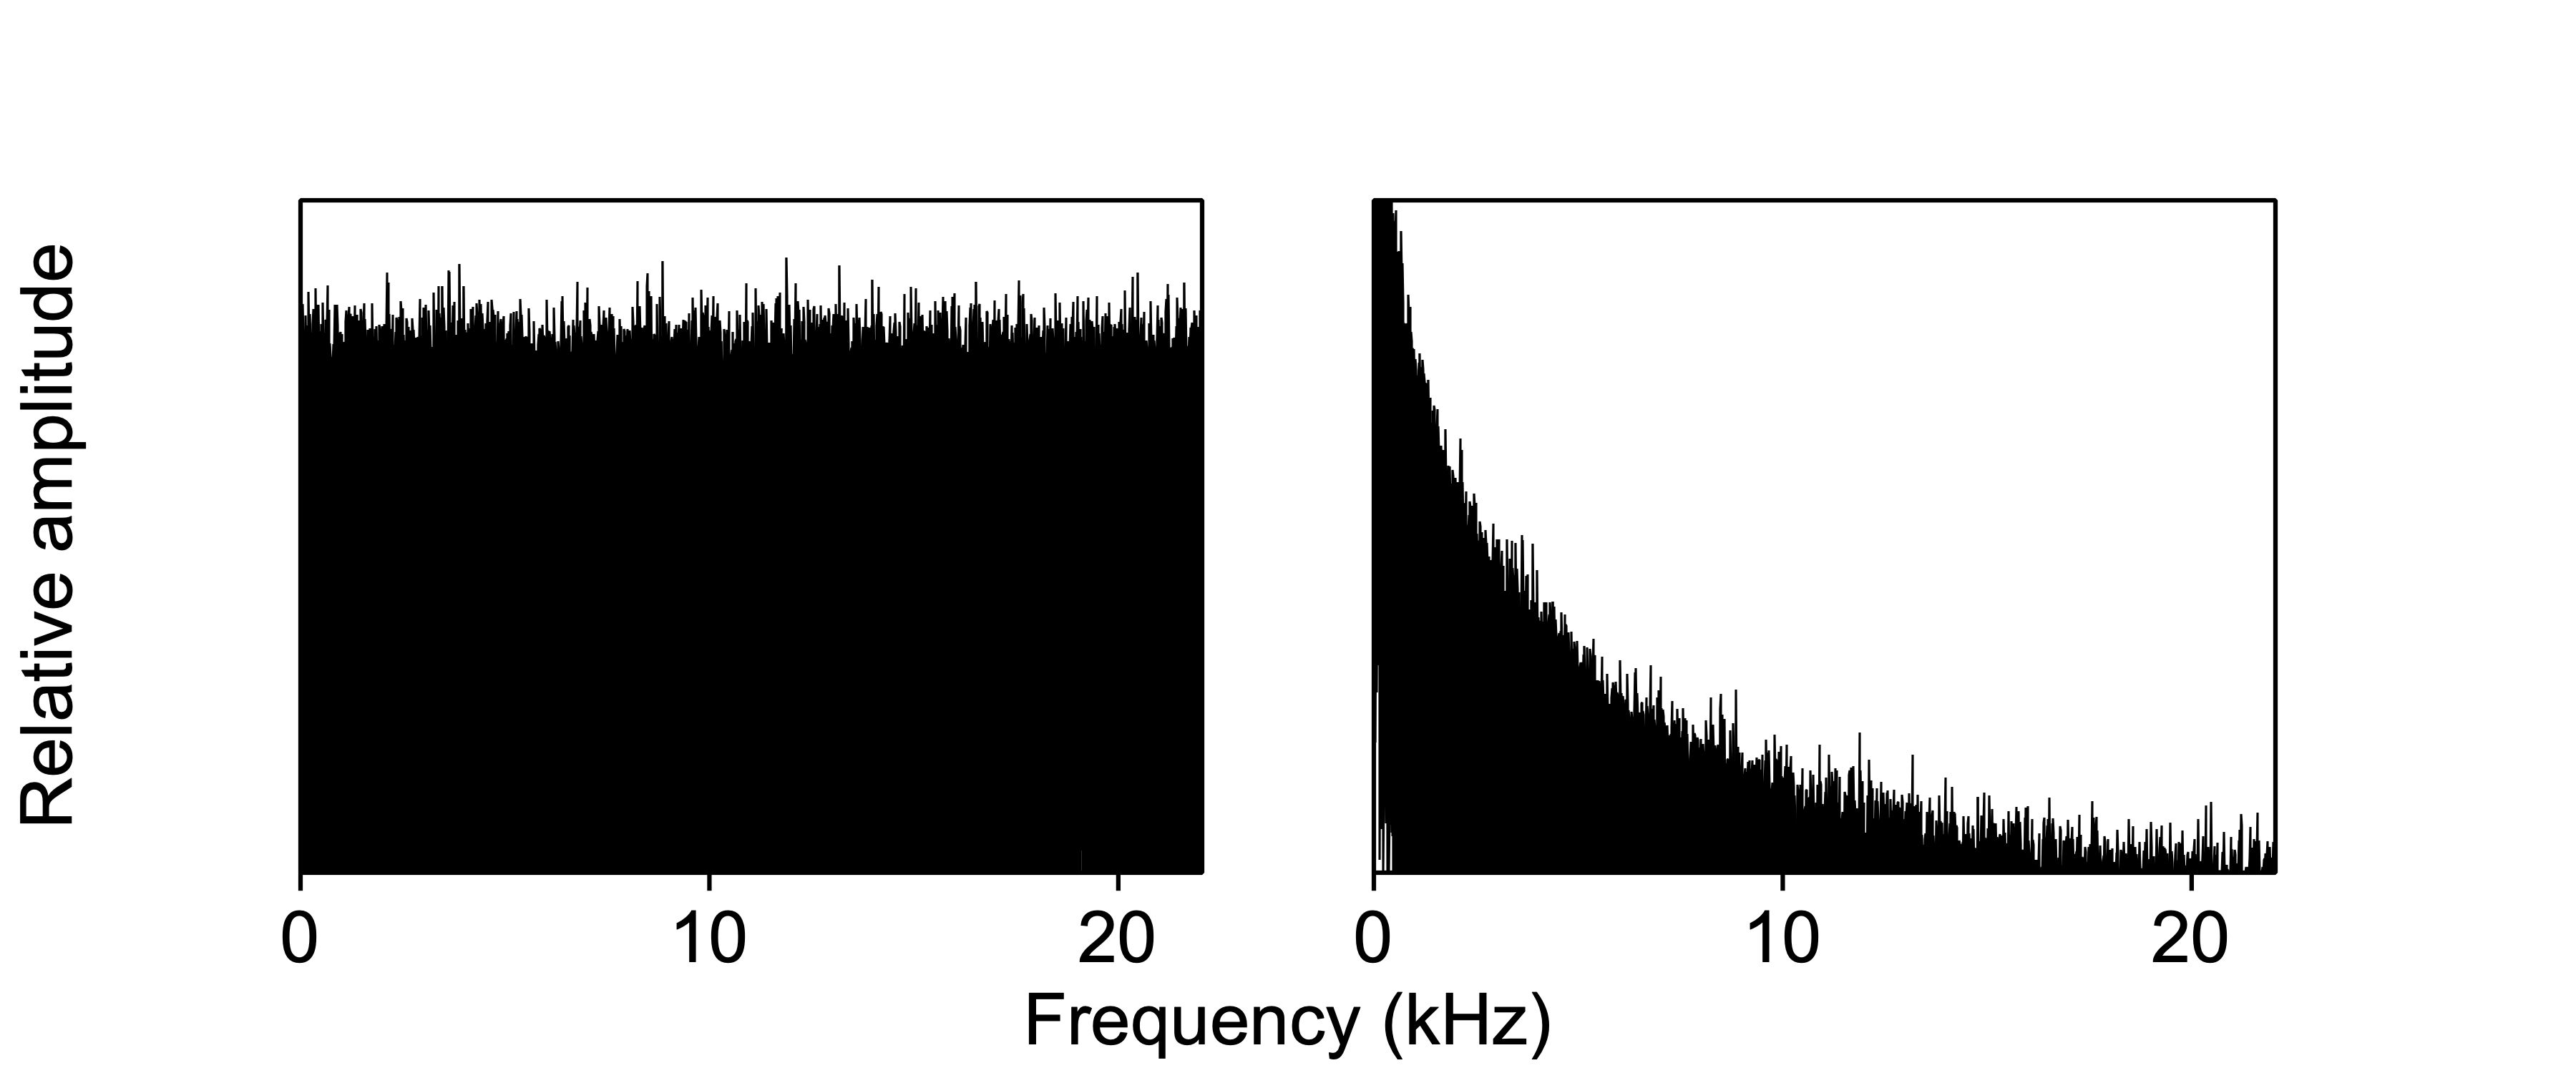
\includegraphics{figures/whitebrownnoises} 

}

\caption{Spectra of white noise (left) and of brown noise (right), with a linear frequency axis (in kHz).}\label{fig:spectrum-whitebrownnoises}
\end{figure}

The random deviations from the ideal, smooth spectral envelope are due to (a) the random variability inherent in noise, and (b) the fact that the spectrum was calculated over a finite amount of time\footnote{If you would listen to white noise for an infinitely long time, then all frequency components would indeed be equally strong.}, with (c) a particular sampling frequency of the noise.

\subsection{Impulses}\label{sec:impulses}

An \textbf{impulse} is a very brief and \emph{transient} sound, such as a hand clap or tick. Acoustically, a very brief impulse sound is like a brief burst of white noise, with a flat spectral envelope. The shorter the impulse, the flatter the spectral envelope becomes.

An impulse may occur unintentionally if the amplitude suddenly increases from zero to a high value, e.g.~at the onset of a sound recording starting at a nonzero value. The resulting noise burst should be effectively removed by \emph{fading in} the sound, see §\ref{sec:fades} for more.

\section{Envelope}\label{envelope}

The \emph{envelope} of a sound describes how the properties of that sound change over time. This concept is best described by regarding the amplitude of a sound: the `amplitude envelope'. However, a sound may at the same time have multiple and different envelopes for its amplitude, for its (fundamental) frequency, and for (a singular parameter of) its timbre. Even the properties of a filter may follow an envelope, that is, they may change over time (see Ch. \ref{ch-filtering}).

The concept of the \emph{envelope} of a sound property stems from electronic music (synthesizers); critical time points are the onset and offset of a key being pressed on the keyboard of the synthesizer. However, the envelope is also a helpful concept for describing analog musical sounds (e.g.~picking a guitar string) and speech sounds (e.g.~plosive vs fricative consonants).

\begin{figure}

{\centering 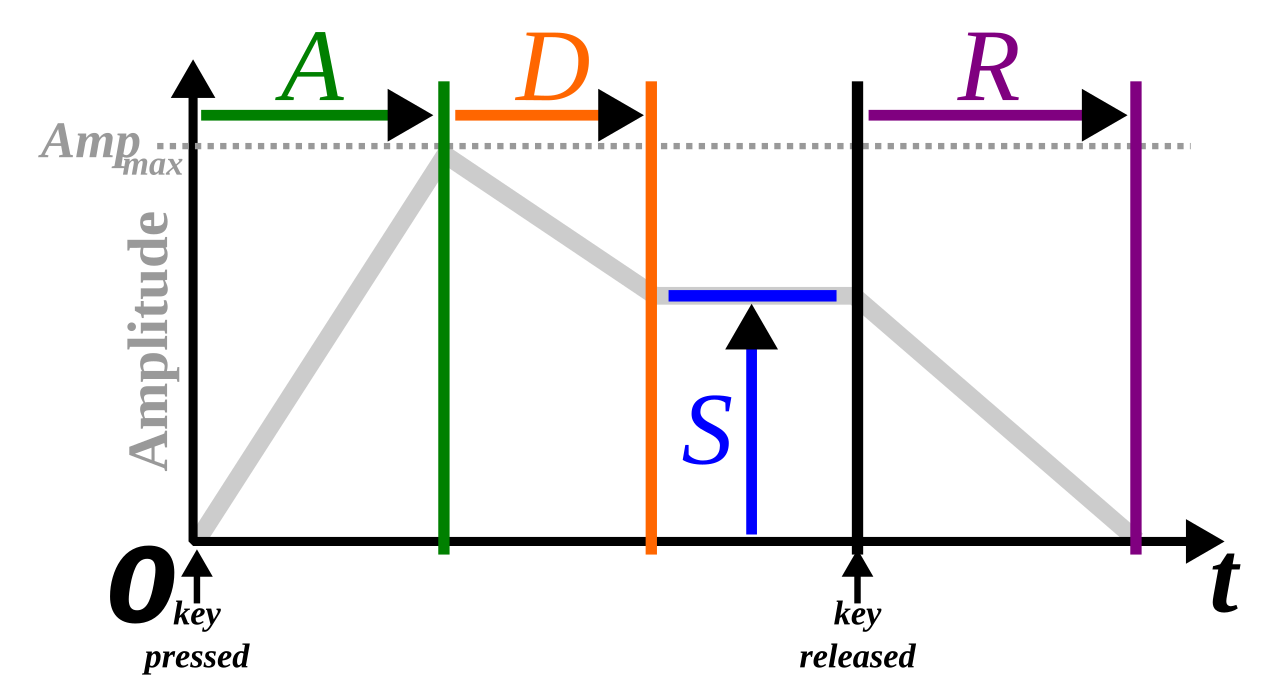
\includegraphics{figures/ADSR_parameter} 

}

\caption{A typical amplitude envelope (in gray), with four key parameters Attack, Decay, Sustain, Release describing the changes of amplitude over time, relative to the onset and offset of a synthesizer keyboard key press. Image taken from  $https://commons.wikimedia.org/wiki/File:ADSR_parameter.svg$, used under CC-BY-SA license.}\label{fig:envelope}
\end{figure}

\begin{quote}
TODO: add text
\end{quote}

\begin{quote}
A
D
S
R
\end{quote}

In terms of its amplitude, we may regard a brief impulse sound (click or pulse, see §\ref{sec:impulses} above) as having very short attack and decay times, a zero sustain level, and zero release time.

\chapter{Filtering}\label{ch-filtering}

\emph{Chapter keywords}: TBA

\section{Introduction}\label{introduction-1}

A filter is a device that changes the spectrum of the input signal, by enhancing certain frequency components and/or by attenuating others. Filters play an important role in speech analysis. Filters can be of an acoustic nature (e.g.~an organ pipe, or the human vocal tract) or they can work by electronic means. We already encountered filters as a routine component in (or just before) analog-to-digital conversion of a sound wave (§\ref{sec:samplingfrequency}) to prevent aliasing.

\section{Types of filters}\label{sec:typesoffilters}

There are four different basic types of filters, differing in their frequency characteristics (specifying which frequency components are attenuated and which are enhanced).

\begin{itemize}
\tightlist
\item
  \textbf{Low-pass} filters (Fig.\ref{fig:lowpassfilter} allow lower frequencies to pass through, but higher frequencies are attenuated.
\end{itemize}

\begin{figure}

{\centering 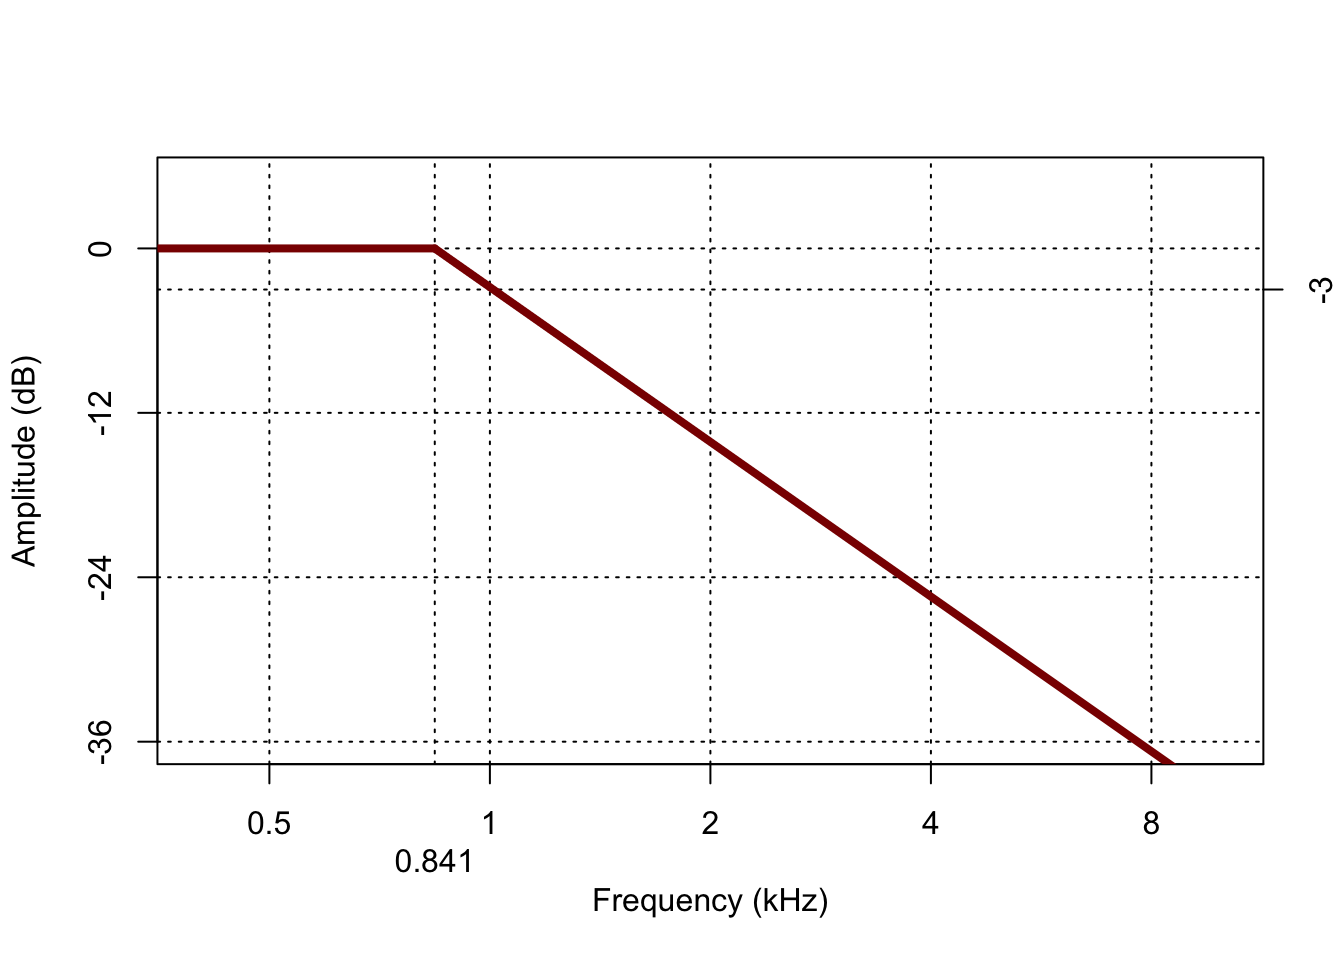
\includegraphics{TPhSA-EN_files/figure-latex/lowpassfilter-1} 

}

\caption{Frequency characteristic of a low-pass filter, with cutoff frequency 1000 Hz, and slope of -12 dB per octave.}\label{fig:lowpassfilter}
\end{figure}

\begin{itemize}
\tightlist
\item
  \textbf{high-pass filters} (Fig.\ref{fig:highpassfilter}) do the reverse: they allow higher frequencies to pass through, but lower frequencies are attenuated.
\end{itemize}

\begin{figure}

{\centering 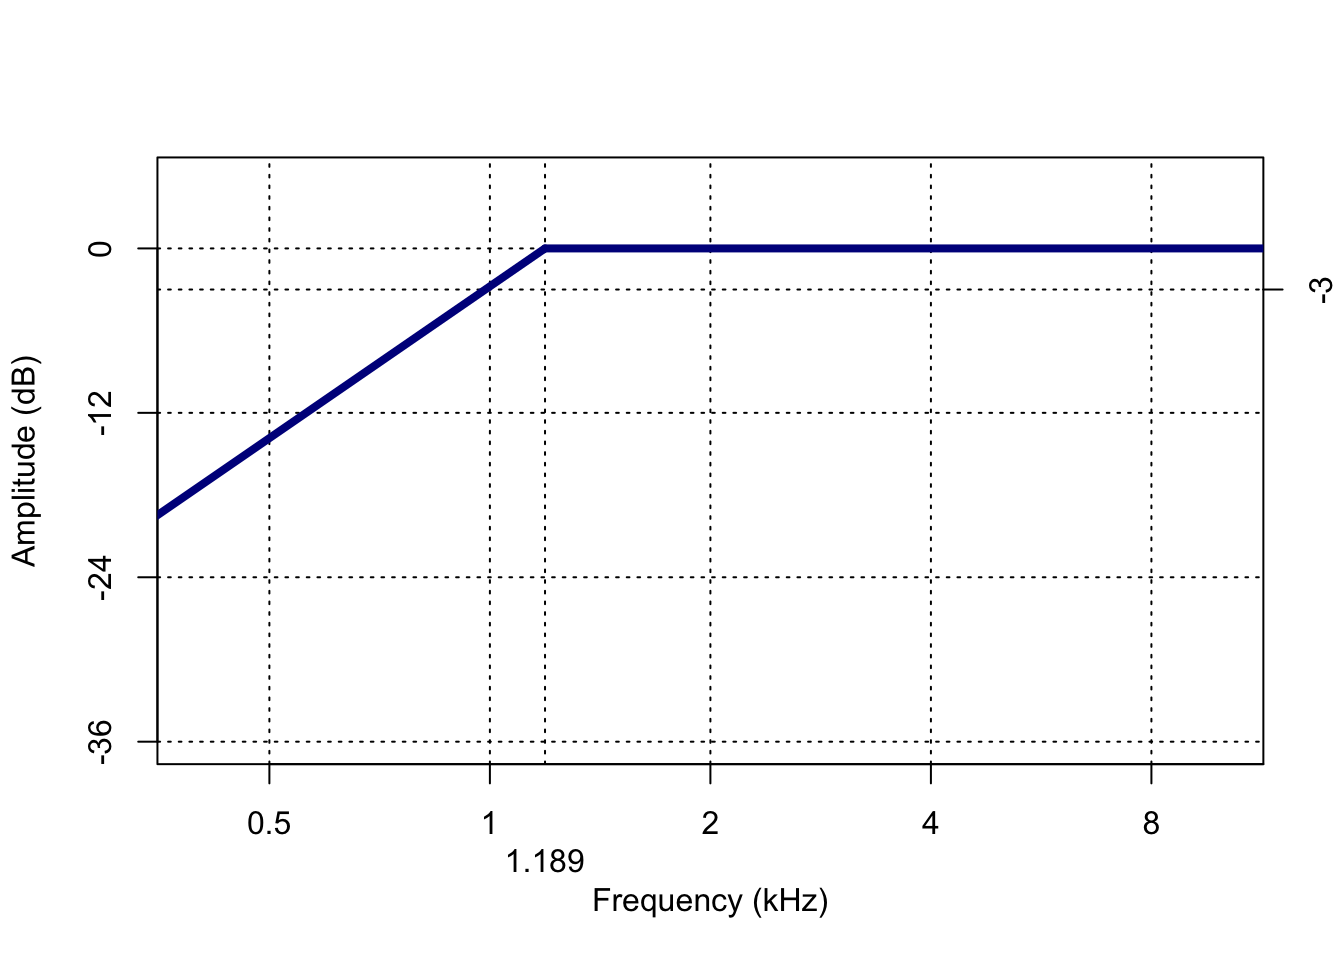
\includegraphics{TPhSA-EN_files/figure-latex/highpassfilter-1} 

}

\caption{Frequency characteristic of a high-pass filter, with cutoff frequency 1000 Hz, and slope of -12 dB per octave.}\label{fig:highpassfilter}
\end{figure}

\begin{itemize}
\tightlist
\item
  \textbf{band-pass filters} (Fig.\ref{fig:bandpassfilter}) allow frequencies within a certain frequency band to pass through, and they attenuate frequencies outside this pass band.
\end{itemize}

\begin{figure}

{\centering 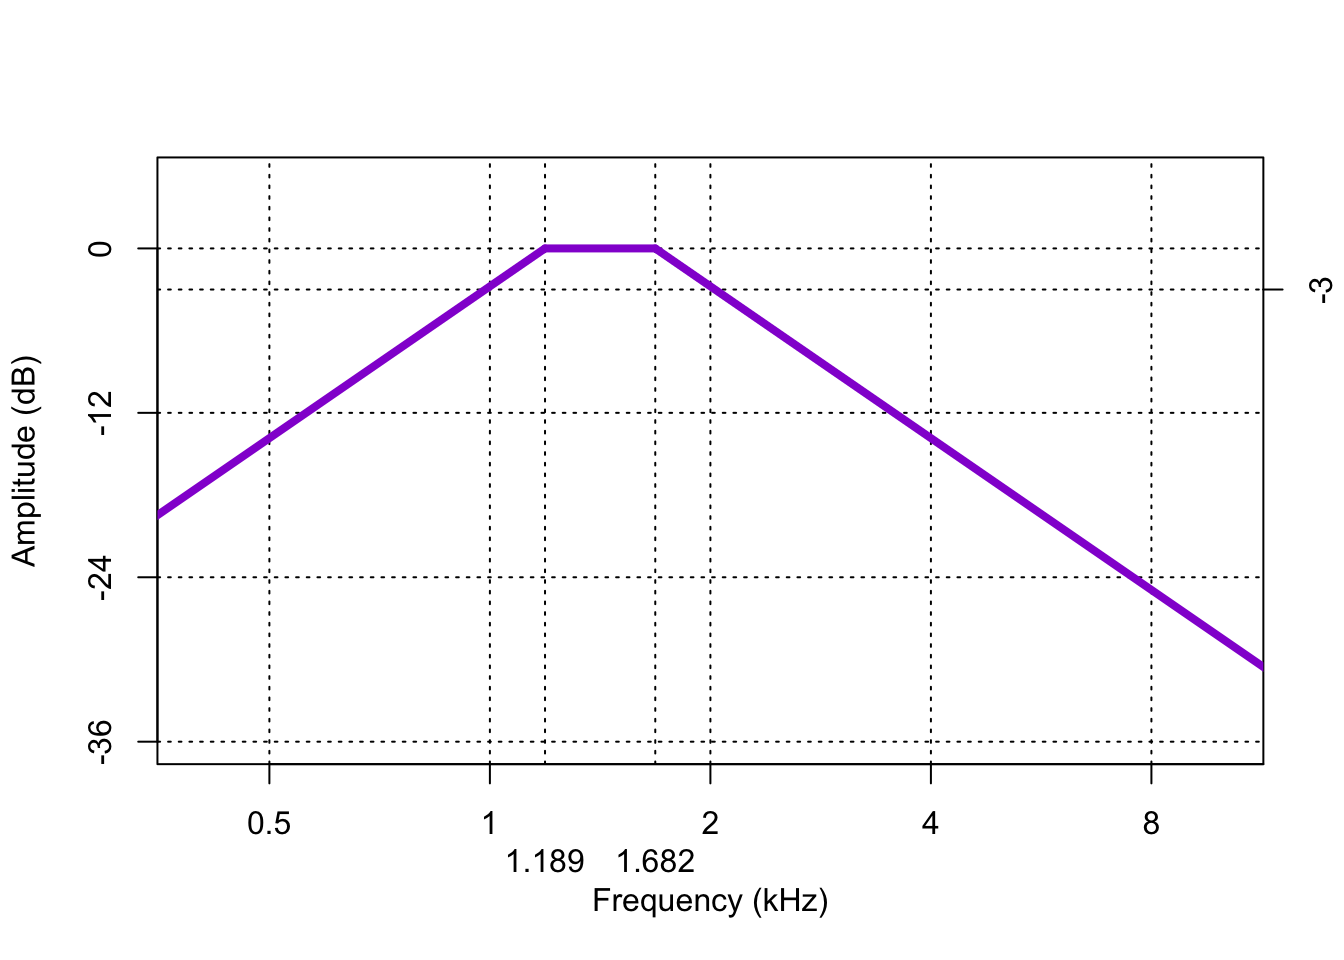
\includegraphics{TPhSA-EN_files/figure-latex/bandpassfilter-1} 

}

\caption{Frequency characteristic of a band-pass filter, with a pass band from 1 to 2 kHz (one octave), and with slopes of -12 dB per octave on both sides.}\label{fig:bandpassfilter}
\end{figure}

-- A tuneable band-pass filter is essential for producing a spectrogram.

\begin{quote}
TODO crossref spectrogram
\end{quote}

-- A telephone works as a bandpass filter with a fixed pass band of 300 to 3400 Hz.

\begin{itemize}
\tightlist
\item
  \textbf{band-reject} or \textbf{notch filters} (Fig.\ref{fig:bandrejectfilter}) again do the reverse: they attenuate frequencies within a certain frequency band, and allow frequencies outside this band to pass through.
\end{itemize}

\begin{figure}

{\centering 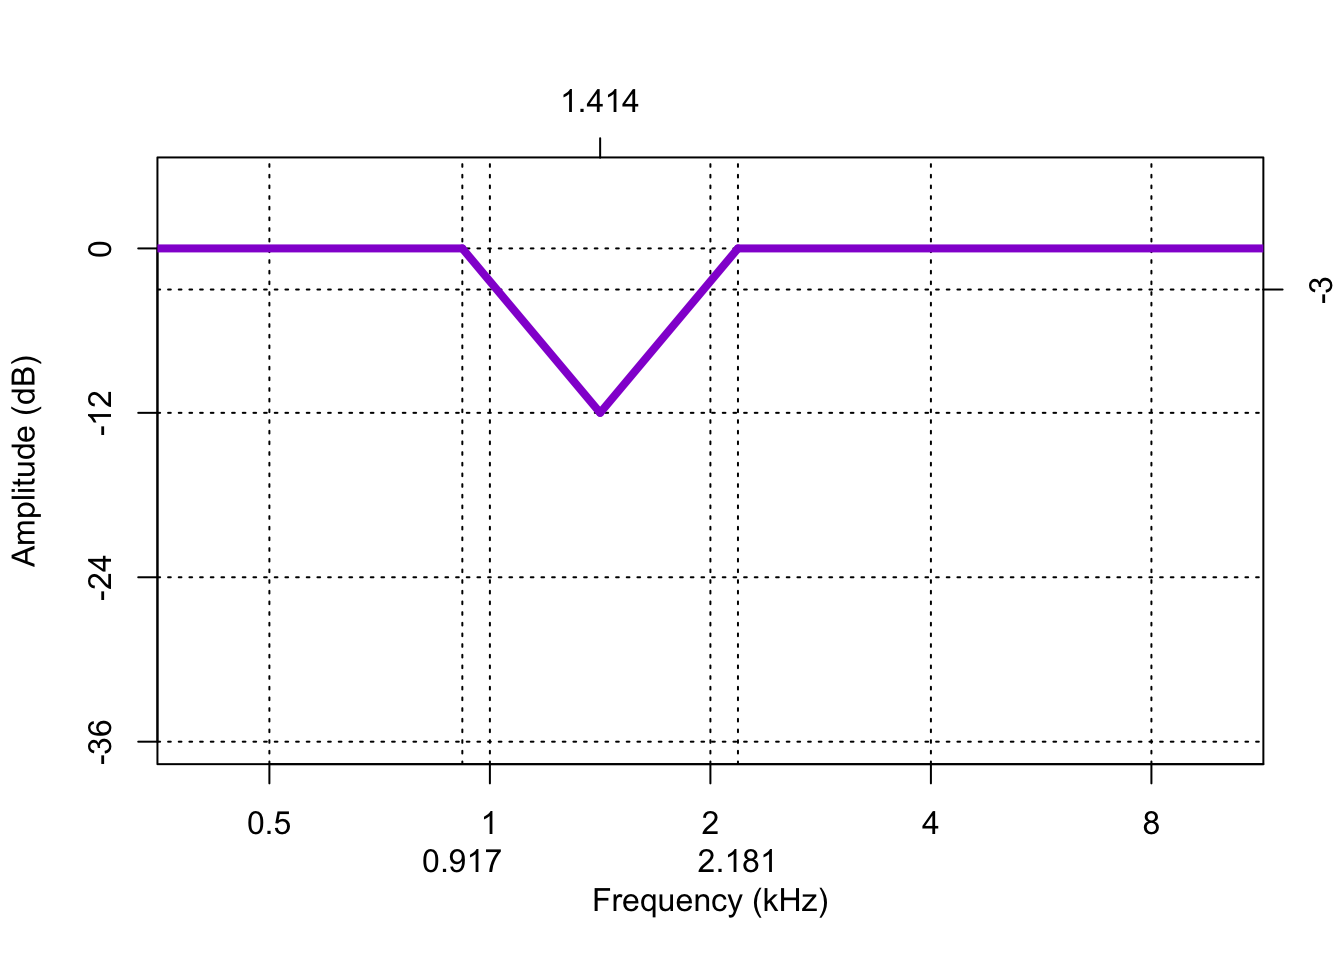
\includegraphics{TPhSA-EN_files/figure-latex/bandrejectfilter-1} 

}

\caption{Frequency characteristic of a band-reject filter, with a reject band from 1 to 2 kHz (one octave), and with slopes of -24 dB per octave on both sides.}\label{fig:bandrejectfilter}
\end{figure}

\section{Properties of filters}\label{properties-of-filters}

As shown in the figures above, a filter is characterised by two properties, viz.~the \emph{cutoff frequency} and the \emph{slope}. Band-pass and band-reject filters are also characterised by their \emph{bandwidth}.

\subsection{Cutoff frequency}\label{cutoff-frequency}

The cutoff frequency(ies) separates the pass band(s) and reject band(s) of the filter, that is, the frequency components that are attenuated and those that are passed through unattenuated. It is defined at the frequency where the attenuation is \(-3\) dB, as illustrated in the filter characteristics above.

\subsection{Slope}\label{slope}

The slope of the filter indicates the steepness of the attenuation between the pass band(s) and reject band(s). It is commonly expressed in dB attenuation per octave change in frequency (§\ref{sec:octave}), that is, in dB per octave\footnote{Note that the band reject filter in Fig.\ref{fig:bandrejectfilter} has steeper slopes than the band pass filter in Fig.\ref{fig:bandpassfilter}.}.

\subsection{Bandwidth}\label{bandwidth}

Band pass filters and band reject filters are also characterised by their bandwidth: the width of the frequency span affected by the filter, equal to the distance between the \emph{two} cutoff frequencies of such filters.

This distance may be expressed as the musical interval between the lower and higher cutoff frequencies. Both filters shown in Figures \ref{fig:bandpassfilter} and \ref{fig:bandrejectfilter} are so-called ``octave band'' filters, because the cutoff frequencies are one octave apart (§\ref{sec:octave}) with a frequency ratio of 1:2.

In a musical third interval, the frequencies have a ratio of 4:5; filters with these cutoff frequency ratios are so-called ``third band'' filters. Both octave-band and third-band filters are widely used in phonetic research.

\section{Emphasis filters}\label{emphasis-filters}

\begin{quote}
TODO crossref source-filter, spectral slope of speech
\end{quote}

For reasons that we will see later (in §REF), the spectrum of speech has a typical overall spectral slope of \(-6\) dB/octave. On average, the amplitude of higher frequency components decreases by about \(-6\) dB for each doubling of the frequency (§\ref{sec:octave}).
Consequently, spectral details of higher-frequency components tend to be poorly visible in the analysis. As a remedy, we can apply a so-called \emph{pre-emphasis} filter, which modifies the overall spectral slope by \(+6\) dB per octave. This boosting of higher-frequency components ideally results in a flat spectral envelope of speech\footnote{The overall average slope of the spectral envelope of speech changes from \(-6\) to \(-6+6=0\) dB per octave.}, with equal amplitudes for all frequency components in speech. This makes the spectral details of speech equally discernible across the full spectral range.

The reverse operation is called \emph{de-emphasis} filtering: this changes the overall spectral slope by \(-6\) dB/octave. This de-emphasis filtering was applied, for example, to obtain the brown noise (\(-6\) dB/oct) from the white noise (\(0\) dB/oct) in Fig.\ref{fig:spectrum-whitebrownnoises}.

\phantomsection\label{box-praatemphasis}
\subsection{How to apply a (pre\textbar de)emphasis filter}\label{how-to-apply-a-predeemphasis-filter}

Select an input Sound object in the \texttt{Praat} Objects window. Then choose \texttt{Filter\ \textgreater{}\ Filter\ (pre-emphasis)...} for pre-emphasis filtering, or choose \texttt{Filter\ \textgreater{}\ Filter\ (de-emphasis)...} for de-emphasis filtering. The filter only applies above a certain cutoff frequency, to be specified. Choose a cutoff frequency below the lowest speech frequency, e.g.~70 Hz.\\
The resulting filtered output Sound object is again added at the bottom of the list of objects.

  \bibliography{book.bib,packages.bib,pandoc.bib,tphsa.bib}

\end{document}
